\documentclass[a4paper,showframe,11pt,draft]{report}
\usepackage{standalone}
\standalonetrue
\ifstandalone
  \usepackage{../../haziq_thesis}
  \usepackage{../../haziq_maths}
  \usepackage{../../haziq_glossary}
  \addbibresource{../../bib/haziq.bib}
  \externaldocument{../01/.texpadtmp/introduction}
\fi

\begin{document}
\hChapterStandalone[2]{Vector space of functions}

One of the main assumptions for regression modelling with I-priors is that the regression functions lie in some vector space of functions.
At first glance, this may seem strange, that the notion of functions (as mappings from input to output space) and vector spaces are somehow equatable.
Upon further thought, one realises that firstly, two functions of a similar, particular form may be added together (in some meaningful way) resulting in a function in that same form. 
Secondly, multiplication of a function by a scalar $c$ can be thought of as $c$ times the output of that function.
Indeed, running through the checklist\footnotemark~of what constitutes a vector space, we find that a ``space of functions'' satisfies them all.
\footnotetext{In modern linear algebra texts, this is the eight axioms of vector spaces over a field $\bbF$: The vectors forms an abelian group under addition, and this group has an $\bbF$-module structure.}

The purpose of this chapter is to provide a concise review of functional analysis leading up to the theory of reproducing kernel Hilbert and Krein spaces (RKHS/RKKS).
The interest with these RKHS and RKKS is that these spaces have well-established mathematical structure and offer desirable topologies.
In particular, it allows the possibility of deriving the Fisher information for regression functions---this will be covered in Chapter 3.
As we shall see, RKHS are also extremely convenient in that they may be specified completely via their reproducing kernels.
Several of these function spaces are of interest to us, for example, spaces of linear functions, smoothing functions, and functions whose inputs are nominal values and even functions themselves.
RKHS are widely studied in the literature, but perhaps RKKS are less so.
To provide an early insight, RKKS are simply an extension of RKHS when its kernel is not positive-definite.
The flexibility provided by RKKS will prove both useful and necessary, especially when considering scaled function spaces, as I-prior modelling does.

It is emphasised that a deep knowledge of functional analysis, including RKHS and RKKS theory, is not at all necessary for I-prior modelling, so perhaps the advanced reader may wish to skip Sections 2.1--2.3. 
Section 2.4 describes the fundamental RKHS of interest for I-prior regression, which we refer to as the ``building block'' RKHS/RKKS.
The reason for this is that it is possible to construct new RKKS from existing ones, and this is described in Section 2.5.

A remark on notation: Elements of the vector space $\cF$ of real functions over a set $\cX$ are denoted $f(\cdot)$, or simply $f$.
This distinguishes them from the actual evaluation of the function at an input point $x \in \cX$, denoted $f(x) \in \bbR$.
For a much cleaner read, we dispense with boldface notation for vectors and matrices when talking about them, without ambiguity, in the abstract sense. 

\section{Some functional analysis}
The core study of functional analysis revolves around the treatment of functions as objects in vector spaces over a field\footnote{In this thesis, this will be $\bbR$ exclusively.}.
Vector spaces, or linear spaces as they are sometimes known, may be endowed with some kind of structure so as to allow ideas such as closeness and limits to be conceived.
Of particular interest to us is the structure brought about by \emph{inner products}\index{inner product}, which allow the rigorous mathematical study of various geometrical concepts such as lengths, directions, and orthogonality, among other things.
We begin with the definition of an inner product. 

\begin{definition}[Inner products]\label{def:innerprod}
	Let $\mathcal F$ be a vector space over $\mathbb R$. A function $\langle\cdot,\cdot\rangle_{\mathcal F}:\mathcal F \times \mathcal F \rightarrow \mathbb R$ is said to be an inner product on $\mathcal F$ if all of the following are satisfied:
	\begin{itemize}
	\item \textbf{Symmetry:} $\langle f, g\rangle_{\mathcal F} = \langle g, f	\rangle_{\mathcal F}$, $\forall f,g \in \mathcal F$.
	\item \textbf{Linearity:} $\langle a f_1 + b f_2, g\rangle_{\mathcal F} = a\langle f_1,g \rangle_{\mathcal F} + b\langle f_2,g \rangle_{\mathcal F}$, $\forall f_1, f_2, g \in \mathcal F$ and $\forall a,b \in \mathbb R$.
	\item \textbf{Non-degeneracy:} $\langle f, f\rangle_{\mathcal F} = 0 \Leftrightarrow f=0$.
%	\item \textbf{Positive-definiteness:} $\langle f, f\rangle_{\mathcal F} \geq 0$, $\forall f \in \mathcal F$.
	\end{itemize}
%	Conversely, an inner product is said to be \emph{negative definite} if $\langle f, f\rangle_{\mathcal F} \leq 0$, $\forall f \in \mathcal F$. 
%	An inner product is said to be \emph{indefinite} it is neither positive nor negative definite.
\end{definition}

Additionally, an inner product is said to be \emph{positive definite} if $\langle f, f\rangle_{\mathcal F} \geq 0$, $\forall f \in \mathcal F$.
It is possible that this may not be the case, and we shall revisit this fact later when we cover Krein spaces.
For the purposes of the discussion moving forward, we shall refer to positive definite inner products, unless otherwise stated.

We can always define a \emph{norm} on $\cF$ using the inner product as 
\begin{align}\label{eq:normip}
  \norm{f}_\cF = \sqrt{\ip{f,f}_\cF}.
\end{align}
%In the above definition we had used the term \emph{norm}.
Norms are another form of structure that specifically captures the notion of length. 
This is defined below.

\begin{definition}[Norms]
	Let $\mathcal F$ be a vector space over $\mathbb R$. A non-negative function $||\cdot||_{\mathcal F}:\mathcal F \times \mathcal F \rightarrow \mathbb [0,\infty)$ is said to be a norm  on $\mathcal F$ if all of the following are satisfied:
	\begin{itemize}
	\item \textbf{Absolute homogeneity:} $||\lambda f||_{\mathcal F} = |\lambda| \cdot ||f||_{\mathcal F}$, $\forall \lambda \in \mathbb R$, $\forall f \in \mathcal F$
	\item \textbf{Subadditivity:} $||f+g||_{\mathcal F} \leq ||f||_{\mathcal F} + ||g||_{\mathcal F}$, $\forall f,g \in \mathcal F$
	\item \textbf{Point separating:} $||f||_{\mathcal F} = 0 \Leftrightarrow f=0$
	\end{itemize}
\end{definition}

\index{subadditivity}\index{inequality!triangle}
The subadditivity property is also known as the \emph{triangle inequality}.
Also note that since $\norm{-f}_\cF = \norm{f}_\cF$, and by the triangle inequality and point separating property, we have that $\norm{f}_\cF + \norm{-f}_\cF \geq \norm{f - f}_\cF = \norm{0}_\cF = 0$, thus implying non-negativity of norms.
Several important relationships between norms and inner products hold in linear spaces, namely, the \emph{Cauchy-Schwarz inequality}\index{inequality!Cauchy-Schwarz}
\[
  |\ip{f,g}_\cF| \leq \norm{f}_\cF\cdot\norm{g}_\cF;
\]
the \emph{parallelogram law}
\[
  \norm{f+g}_\cF^2 - \norm{f+g}_\cF^2 = 2\norm{f}_\cF^2 + 2\norm{g}_\cF^2;
\]
and the \emph{polarisation identity}
\[
  \norm{f+g}_\cF^2 + \norm{f+g}_\cF^2 = 4\ip{f,g}_\cF,
\]
for some $f,g\in\cF$.

A vector space endowed with an inner product (c.f. norm) is called an inner product space (c.f. normed vector space).
%A normed vector space is a vector space whose vectors have lengths, as induced by its norm.
As a remark, inner product spaces can always be equipped with a norm using \eqref{eq:normip}, but not always the other way around.
A norm needs to satisfy the parallelogram law for an inner product to be properly defined.

The norm $||\cdot||_{\mathcal F}$, in turn, induces a metric (a notion of distance) on $\mathcal F$: $d(f,g) = ||f-g||_{\mathcal F}$, for $f,g\in\cF$.
With these notions of distances, one may talk about sequences of functions in $\cF$ which are \emph{convergent}, and sequences whose elements become arbitrarily close to one another as the sequence progresses (\emph{Cauchy}).

\begin{definition}[Convergent sequence]
	A sequence $\{f_n\}_{n=1}^\infty$ of elements of a normed vector space $(\mathcal F, ||\cdot ||_{\mathcal F})$ is said to be \emph{converge} to some $f\in\cF$, if for every $\epsilon > 0$, $\exists N=N(\epsilon) \in \mathbb N$, such that $\forall n > N$, $||f_n - f||_{\mathcal F} < \epsilon$.
\end{definition}

\begin{definition}[Cauchy sequence]
	A sequence $\{f_n\}_{n=1}^\infty$ of elements of a normed vector space $(\mathcal F, ||\cdot ||_{\mathcal F})$ is said to be a Cauchy sequence if for every $\epsilon > 0$, $\exists N=N(\epsilon) \in \mathbb N$, such that $\forall n,m > N$, $||f_n - f_m||_{\mathcal F} < \epsilon$.
\end{definition}

Every convergent sequence is Cauchy (from the triangle inequality), but the converse is not true.
If the limit of the Cauchy sequence exists within the vector space, then the sequence converges to it.
If the vector space contains the limits of all Cauchy sequences (or in other words, if every Cauchy sequence converges), then it is said to be \emph{complete}.
On the other hand, a set which contains all of its limit points is said to be \emph{closed}.
Clearly, a complete set must closed, but a closed set need not necessarily be complete.

There are special names given to complete vector spaces.
A complete inner product space is known as a \emph{Hilbert space}, while a complete normed space is called a \emph{Banach space}.
Out of interest, an inner product space that is not complete is sometimes known as a \emph{pre-Hilbert space}, since its completion with respect to the norm induced by the inner product is a Hilbert space.

Being vectors in a vector space, we can discuss mapping the vectors onto a different space, or in essence, having a function acted upon them.
To establish terminology, we define linear functionals, bilinear form, and linear operators.

\begin{definition}[Linear functional]
  Let $\cF$ be a Hilbert space.
  A \emph{functional} $L$ is a map from $\cF$ to $\bbR$, and we denote its action on a function $f$ as $L(f)$. 
  A functional is called \emph{linear} if it satisfies $L(f+g)=L(f)+L(g)$ and $L(\lambda f)=\lambda L(f)$, for all $f,g\in\cF$ and $\lambda\in\bbR$.
\end{definition}

\begin{definition}[Bilinear form]
  Let $\cF$ be a Hilbert space.
  A \emph{bilinear form} $B$ takes inputs $f,g\in\cF$ and returns a real value.
  It is linear in each argument separately, i.e.
  \begin{itemize}
    \item $B(\lambda_1 f +\lambda_2 g, h) = \lambda_1 B(f,h) + \lambda_2 B(g,h)$; and
    \item $B(f, \lambda_1 g +\lambda_2 h) = \alpha B(f,g) + \lambda_2 B(f,h)$,
  \end{itemize} 
  for all $f,g,h \in \cF$ and $\lambda_1,\lambda_2\in\bbR$.
\end{definition}

\begin{definition}[Linear operator]
  Let $\cF$ and $\cG$ be two Hilbert spaces over $\bbR$.
  An operator $A$ is a map from $\cF$ to $\cG$, and we denote its action on a function $f \in\cF$ as $Af \in \cG$.
  A \emph{linear operator} satisfies $A(f+g) = A(f) + A(g)$ and $A(\lambda f) = \lambda A(f)$, for all $f,g \in\cF$ and $\lambda\in\bbR$.
\end{definition}

The term `functional' is classically used in calculus of variations to denote `a function of a function', i.e. a function having another function as its input, and outputs a real number.
Really, from a function space perspective, it is simply a mapping of functions onto another vector space (the reals in this case).
More generally, if the output space is another Hilbert space, then it is an operator.
An interesting property of these operators to look at, besides linearity, is whether or not they are \emph{continuous}.

\index{continuous}
\index{continuous!uniform}
\begin{definition}[Continuity]\label{def:continuity}
  Let $\cF$ and $\cG$ be two Hilbert spaces.
  A function $A:\cF\to\cG$ is said to be \emph{continuous at $g\in\cF$}, if for every $\epsilon>0$, $\exists \delta=\delta(\epsilon,g)>0$ such that
  \[
    \norm{f-g}_\cF < \delta \ \ \Rightarrow \ \ \norm{Af - Ag}_\cG < \epsilon.
  \]
  A is \emph{continuous} on $\cF$, if it is continuous at every point $g \in\cF$.
  If, in addition, $\delta$ depends on $\epsilon$ only, $A$ is said to be \emph{uniformly continuous}.
\end{definition}

Continuity in the sense of linear operators here means that a convergent sequence in $\cF$ can be mapped to a convergent sequence in $\cG$.
For a special case of linear operator, the evaluation functional, this means that a function in $\cF$ is continuous if the evaluation functional is continuous---more on this later in Section \ref{sec:rkhstheory}.
There is an even stronger notion of continuity called the \emph{Lipschitz continuity}.

\begin{definition}[Lipschitz continuity]
  Let $\cF$ and $\cG$ be two Hilbert spaces.  
  A function $A:\cF\to\cG$ is \emph{Lipschitz continuous} if $\exists M >0$ such that $\forall f,f'\in\cF$,
  \[
    \norm{Af - Af'}_\cG \leq M \norm{f - f'}_\cF.
  \]
\end{definition}

Clearly, Lipschitz continuity implies uniform continuity: Choose $\delta = \delta(\epsilon) := \epsilon/M$ and replace this in Definition \ref{def:continuity}.
So important is the concept of linearity and continuity, that there are specially named spaces which contain linear and continuous functionals.

\begin{definition}[Dual spaces]
  Let $\cF$ be a Hilbert space. 
  The space $\cF^*$ of \emph{linear functionals} is called the \emph{algebraic dual space} of $\cF$.
  The space $\cF'$ of \emph{continuous linear functionals} is called the \emph{continuous dual space} or alternatively, the \emph{topological dual space}, of $\cF$.   
\end{definition}

As it turns out, the algebraic dual space and continuous dual space coincide in finite-dimensional Hilbert spaces:
Take any $L\in\cF'$; since $L$ is finite-dimensional, it is bounded, and therefore continuous (see Lemma \ref{thm:boundcont}) so $L\in\cF'$ and $\cF^* \subseteq \cF'$; but $\cF' \subseteq \cF^*$ trivially, so $\cF^* \equiv \cF'$.
For infinite-dimensional Hilbert spaces, this is not so, but in any case, we will only be considering the continuous dual space in this thesis.

\begin{definition}[Bounded operator]\label{def:boundedop}
  The linear operator $A:\mathcal F \rightarrow \mathcal G$ between two Hilbert spaces $\cF$ and $\cG$ is said to be \emph{bounded} if there exists some $M>0$ such that
  \[
    \norm{Af}_\cG \leq M \norm{f}_\cF.
  \] 
  The smallest such $M$ is defined to be the \emph{operator norm}, denoted $\norm{A} := \sup_{f\in\cF} \frac{\norm{Af}_\cG}{\norm{f}_\cF}$.
\end{definition}

\begin{lemma}[Equivalence of boundedness and continuity]\label{thm:boundcont}
  Let $\cF$ and $\cG$ be two Hilbert spaces, and $A:\cF\to\cG$ a linear operator.
  $A$ is a bounded if and only if it is continuous.
\end{lemma}

\begin{proof}
  Suppose that $L$ is bounded.
  Then, $\forall f,f' \in \cF$, there exists some $M>0$ such that $\norm{A(f-g)}_\cG \leq M \norm{f-g}_\cG.$
  Conversely, let $A$ be a continuous linear operator, especially at the zero vector.
  In other words, $\exists \delta > 0$ such that $\norm{A(f)}_\cG = \norm{A(f+0-0)}_\cG = \norm{A(f) - A(0)} \leq 1$, $\forall f\in\cF$ whenever $\norm{f}_\cF \leq \delta$.
  Thus, for all non-zero $f \in\cF$,
  \begin{align*}
    \norm{A(f)}_\cG &= \left\Vert \frac{\norm{f}_\cF}{\delta} A\left(\frac{\delta}{\norm{f}_\cF}f\right)\right\Vert_\cG \\
    &= \left\vert \frac{\norm{f}_\cF}{\delta}\right\vert \cdot \left\Vert A\left(\frac{\delta}{\norm{f}_\cF}f\right)\right\Vert_\cG \\    
    &\leq \frac{\norm{f}_\cF}{\delta} \cdot 1,
  \end{align*}
  and thus $A$ is bounded.
\end{proof}

The following result is an important one, which states that (continuous) linear functionals of an inner product space are nothing more than just inner products.

\begin{theorem}[Riesz representation]
  Let $\cF$ be a Hilbert space.
  Every element $L$ of the continuous dual space $\cF'$, i.e. all continuous linear functionals $L:\cF\to\bbR$, can be uniquely written in the form $L=\ip{\cdot,g}_\cF$, for some $g\in\cF$.
\end{theorem}

\begin{proof}
  Omitted---see \citet[Theorem 4.12]{rudin1987real} for a proof.
\end{proof}

\begin{corollary}[Riesz norm]
  For any $f\in\cF$ a Hilbert space, define $L(f) = \ip{f,g}_\cF$ for some $g\in\cF$.
  Then $\norm{L}_{\cF'} = \norm{g}_\cF$. 
\end{corollary}

\begin{proof}
%  $L$ as defined by $L = \ip{\cdot,g}_\cF$ for some $g\in\cF$ is a linear operator $L:\cF\to\cF'$,
%  so from Definition \ref{def:boundedop} of operator norms,
%  \begin{align*}
%    \norm{L} &= \sup_{f\in\cF} \frac{\norm{L(f)}_{\cF'}}{\norm{f}_\cF} \\
%    &= \sup_{f\in\cF} \frac{|\ip{f,g}_{\cF}|}{\norm{f}_\cF} \\
%    &=  \frac{|\ip{g,g}_{\cF}|}{\norm{g}_\cF} \\
%    &= \norm{g}_\cF
%  \end{align*}
%  by the Cauchy-Schwarz inequality.
%  Alternative proof:
  By Cauchy-Schwarz,
  \[
    |L(f)| \leq \norm{f}_\cF\norm{g}_\cF
  \]
  so $\norm{L}_{\cF'}\leq \norm{g}_\cF$.
  But  $|L(g)| = \norm{g}_\cF^2$, so in fact $\norm{L}_{\cF'} = \norm{g}$\hltodo[Not so convinced.]{}
\end{proof}

The notion of isometry (transformation that preserves distance) is usually associated with metric spaces---two metric spaces being isometric means that they identical in as far as their metric properties are concerned.
For Hilbert spaces (or normed spaces in general), there is an analogous concept as well in \emph{isometric isomorphism} (a bijective isometry), such that two Hilbert spaces being isometrically isomorphic imply that they have exactly the same geometric structure, but may very well contain fundamentally different objects.

\begin{definition}[Isometric isomorphism]
  Two Hilbert spaces $\cF$ and $\cG$ are said to be \emph{isometrically isomorphic} if there is a linear bijective map $A:\cF\to\cG$ which preserves the inner product, i.e. 
  \[
    \ip{f,f'}_\cF = \ip{Af,Af'}_\cG.
  \]
\end{definition}

In Hilbert spaces, this isometry is also known as \emph{linear isometry}.
A consequence of the Riesz representation theorem is that it gives us a canonical isometric isomorphism $A:f\mapsto \ip{\cdot,f}_\cF$ between $\cF$ and its continuous dual $\cF'$, whereby $\norm{Af}_{\cF'} = \norm{f}_\cF$.
Implicitly, this means that $\cF'$ is a Hilbert space as well.

Another important type of mapping is the mapping $P$ of an element in $\cF$ onto a closed subspace $\cG\subset\cF$, such that $Pf \in \cG$ is closest to $f$.
This mapping is called the \emph{orthogonal projection}, due to the fact that such projections yield perpendicularity in the sense that $\ip{f-Pf,g}_\cG = 0$ for any $g\in\cG$.
The remainder $f - Pf$ belongs to the \emph{orthogonal complement} of $\cG$.

\begin{definition}[Orthogonal complement]
  Let $\cF$ be a Hilbert space and $\cG \subset \cF$ be a closed subspace.
  The linear subspace $\cG^\bot = \{ f \,|\, \ip{f,g}_\cG = 0, \forall g \in \cG \}$ is called the orthogonal complement of $\cG$.
\end{definition}

\begin{theorem}[Orthogonal decomposition]
  Let $\cF$ be a Hilbert space and $\cG \subset \cF$ be a closed subspace.
  For every $f \in \cF$, we can write $f = g + g^c$, where $g \in \cG$ and $g^c \in \cG^\bot$, and this decomposition is unique.
\end{theorem}

\begin{proof}
  Omitted---see \citet[Theorem 4.11]{rudin1987real} for a proof.
\end{proof}

We can write $\cF = \cG \oplus \cG^\bot$, where the $\oplus$ symbol denotes the \emph{direct sum}, and such a decomposition is called a \emph{tensor sum decomposition}.
In infinite-dimensional Hilbert spaces, some subspaces are not closed, but all orthogonal complements are closed. 
In such spaces, the orthogonal complement of the orthogonal complement of $\cG$ is the closure of $\cG$, i.e. $(\cG^\bot)^\bot =: \overline \cG$, and we say that $\cG$ is dense in $\overline \cG$.
Another interesting fact regarding the orthogonal complement is that $\cG \cap \cG^\bot = \{ 0 \}$, since any $g\in \cG \cap \cG^\bot$ must be orthogonal to itself, i.e. $\ip{g,g}_\cG = 0$ implying that $g=0$.

\begin{corollary}
  Let $\cG$ be a subspace of a Hilbert space $\cF$. 
  Then, $\cG^\bot = \{0\}$ if and only if $\cG$ is dense in $\cF$.
\end{corollary}

\begin{proof}
  If $\cG^\bot=\{0\}$ then $(\cG^\bot)^\bot = \overline \cG = \cF$.
  Conversely, since $\cG$ is dense in $\cF$, we have $\cG^\bot = \overline\cG^\bot = \cF^\bot = \{0\}$.
%  Conversely, suppose that there exists a non-zero element $h \in \cG^\bot$.
%  Because $\cG$ is dense, we can construct a sequence $\{h_n\}_{n=1}^\infty\in\cG$ converging to $h$.
%  We have
%  \begin{align*}
%    \norm{h}_\cG^2 
%    &= \ip{h,h}_\cG \\
%    &= \ip{h,h}_\cG - \ip{h_n,h}_\cG \hspace{1em} \rlap{\color{gray} since $h$ is in $\cG^\bot$} \\
%    &= \ip{h-h_n,h}_\cG \\
%    &\leq \norm{h-h_n}_\cG \cdot \norm{h}_\cG,
%  \end{align*}
%  but the final term tends to zero since $h_n$ converges to $h$.
%  So $h=0$, a contradiction.
\end{proof}

%https://en.wikibooks.org/wiki/Functional_Analysis/Hilbert_spaces

For the last part of this introductory section on functional analysis, we discuss measures on Hilbert spaces, and in particular, a probability measure.
Let $\cX$ be a real topological space (e.g. real Hilbert spaces), and let $\cB(\cX)$ the Borel $\sigma$-algebra of $\cX$.
A measure $\nu$ on $\big(\cX,\cB(\cX)\big)$ is called a \emph{Borel measure} on $\cX$.
We shall only concern ourselves with finite Borel measures. 
If $\nu(\cX) = 1$ then $\nu$ is a \emph{(Borel) probability measure} and the measure space $\big(\cX,\cB(\cX),\nu\big)$ is a \emph{(Borel) probability space}.

\begin{definition}[Mean vector and covariance operator]
  Let $\nu$ be a Borel probability measure on a real topological space $\cX$.
  Supposing that the function $z \mapsto \ip{z,x}_\cX$ is integrable with respect to $\nu$, the element $\mu\in\cX$ satisfying 
  \[
    \ip{\mu,x} = \int_\cX \ip{z,x}_\cX \d\nu(z), \ \forall x \in \cX
  \]
  is called the \emph{mean vector}.
  If, furthermore, there is a positive, symmetric linear operator $C$ on $\cX$ such that
  \[
    \ip{Cx,x'} = \int_\cX \ip{x,z-\mu}_\cX\ip{x',z-\mu}_\cX \d\nu(z), \ \forall x,x' \in \cX,
  \]
  then $C$ is called the \emph{covariance operator}.
  The conditions requiring existence of the mean vector and covariance operator are $\int_\cX |x| \d\nu(x) < \infty$ and $\int_\cX |x|^2 \d\nu(x) < \infty$ respectively.
\end{definition}

\begin{definition}[Mean and covariance of functions]
  Let $\big(\cX,\cB(\cX),\nu\big)$ be a Borel probability space, and let $\phi:\cX\to\cF$ be a feature map of some Hilbert space of functions $\cF$.
  The \emph{mean element} of $\cF$ is defined as $\mu_f \in \cF$ satisfying
  \[
    \E\ip{f,f'}_\cF = \ip{\mu_f,f'}_\cF
  \]
  for all $f'\in\cF$.
  The quantity $\ip{\mu_f,f}_\cF := \E\ip{\phi(x),f}_\cF$ is denoted $\E f(X)$.
\end{definition}

\hltodo{Slightly confused: Do we need random functions $f\in\cF$ or are the covariates $x\in\cX$ assumed to be random? Later on in Section 2.4 and 2.5, we talk about $\E f(X)$ so there is some measure on $\cX$. However, when we prove the I-prior, we talk about $f$ itself being random.}

\hltodo{Also, are Definitions 2.14 and 2.15 similar?}

\hltodo{Covariance is $C \in \cF \otimes \cF$ satisfying $\Cov(\ip{f,g}, \ip{f,g'}) = \ip{C, g\otimes g}$. How does this definition tie in the above?}


\section{Reproducing kernel Hilbert space theory}\label{sec:rkhstheory}
The introductory section sets us up nicely to discuss the coveted reproducing kernel Hilbert space.
This is a subset of Hilbert spaces for which its evaluation functionals are continuous (by definition, in fact).
The majority of this section, apart from defining RKHS, is to convince ourselves that each and every RKHS of functions can be specified solely through its reproducing kernel.
To begin, we consider a fundamental linear functional on a Hilbert space of functions $\cF$, that assigns a value to $f \in \mathcal F$ for each $x \in \mathcal X$.

\begin{definition}[Evaluation functional]
	Let $\mathcal F$ be a vector space of functions $f:\mathcal X \rightarrow \mathbb R$, defined on a non-empty set $\mathcal X$. 
	For a fixed $x \in \mathcal X$, the functional $\delta_x:\mathcal F \rightarrow \mathbb R$ as defined by $\delta_x(f) = f(x)$ is called the (Dirac) evaluation functional at $x$.
\end{definition}

It is easy to see that evaluation functionals are always linear: $\delta_x(\lambda f + g) = (\lambda f + g)(x) = \lambda f(x) + g(x) = \lambda\delta_x(f) + \delta_x(g)$.
This is in fact the linearity that was implied earlier on at the beginning of Chapter 2 when introducing the notion of functions behaving like vectors.
As a remark, the calculation of the (penalised) likelihood functional involves evaluations. 
It is therefore important for the evaluation functional to be continuous.
It turns out, this is exactly what RKHS provide.

\begin{definition}[Reproducing kernel Hilbert space]\label{def:rkhs}
	A Hilbert space $\cF$ of real-valued functions $f:\mathcal X \rightarrow \mathbb R$ on a non-empty set $\mathcal X$ is called a \emph{reproducing kernel Hilbert space} if the evaluation functional $\delta_x: f \mapsto f(x)$ is continuous (equivalently, bounded) on $\cF$, $\forall x \in \cX$. 
\end{definition}

\begin{figure}[hbt]
  \centering
  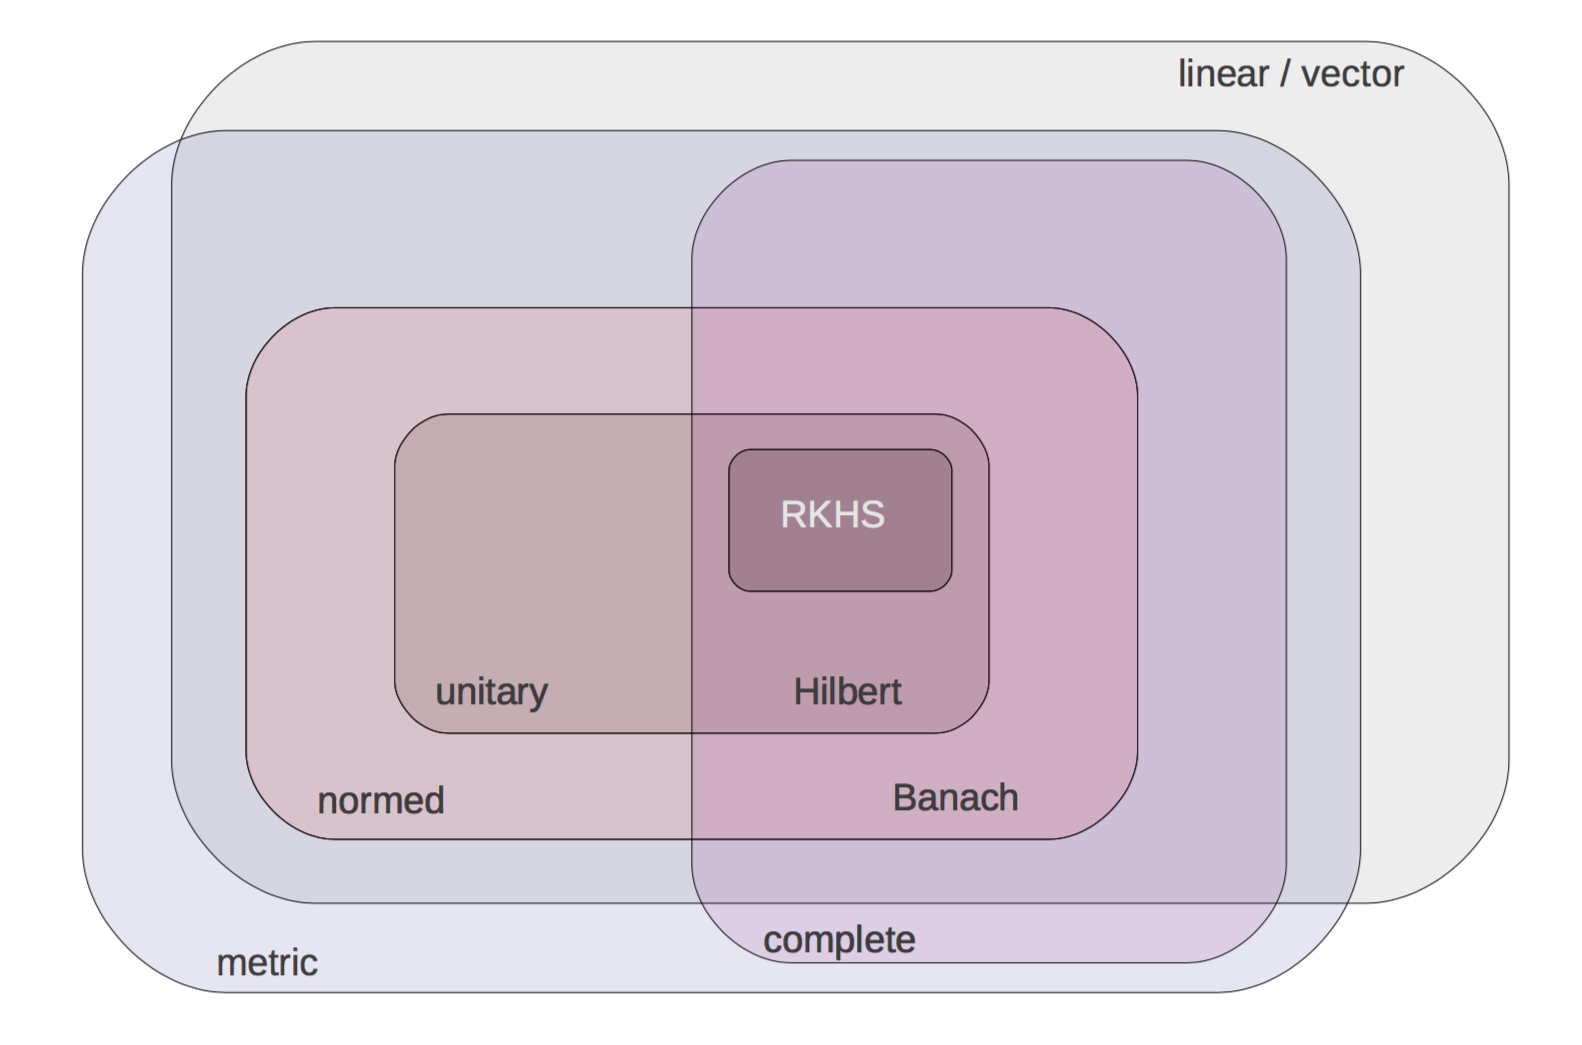
\includegraphics[scale=0.22]{figure/hierarchy-spaces.png}
  \caption{A hierarchy of vector spaces. Reproduced from the lecture slides of Dino Sejdinovic and Arthur Gretton entitled `Foundations of Reproducing Kernel Hilbert Spaces: Advanced Topics in Machine Learning', 2014. URL: \url{www.gatsby.ucl.ac.uk/~dino/teaching}.}
\end{figure}

%The continuity condition also represents the weakest condition required for both the existence of an inner product and the evaluation of every function in $\cF$ at every point in the domain $\cX$.
While the continuity condition by definition is what makes an RKHS, it is neither easy to check this condition in practice, nor is it intuitive as to the meaning of its name.
In fact, there isn't even any mention of what a reproducing kernel actually is.
In order to benefit from the desirable continuity property of RKHS, we should look at this from another, more intuitive, perspective. 
By invoking the Riesz representation theorem, we see that for all $x\in\cX$, there exists a unique element $h_x\in\cF$ such that
\[
  f(x) = \delta_x(f) = \ip{f,h_x}_\cF, \forall f \in \cF
\]
holds. 
Since $h_x$ itself is a function in $\cF$, it holds that for every $x' \in \cX$ there exists a $h_{x'}\in\cF$ such that
\[
  h_{x}(x') = \delta_{x'}(h_{x}) = \ip{h_x,h_{x'}}_\cF.
\]
This leads us to the definition of a \emph{reproducing kernel} of an RKHS---the very notion that inspired its name.

\begin{definition}[Reproducing kernels]\label{def:repkern}
  Let $\mathcal F$ be a Hilbert space of functions over a non-empty set $\mathcal X$. A function $h:\mathcal X\times\mathcal X\rightarrow\mathbb R$ is called a reproducing kernel of $\mathcal F$ if $h$ satisfies
  \begin{itemize}
    \item $\forall x \in \mathcal X,\, h(\cdot, x) \in \mathcal F$; and
    \item $\forall x \in \mathcal X, \, f \in \mathcal F, \, \langle f, h(\cdot, x) \rangle_{\mathcal F} = f(x)$ (the reproducing property).
  \end{itemize}
  In particular, for any $x, x' \in \mathcal X$,
  \[
  	h(x,x') = \langle h(\cdot, x), h(\cdot, x') \rangle_{\mathcal F}.
  \]
\end{definition}

Continuity of evaluation functionals in an RKHS means that functions that are close in RKHS norm imply that they are also close pointwise.
\hltodo[Not so sure why this is useful?]{It gives some reassurance when trying to estimate $f$ from $\cF$---just look at the size of the norm.}
More formally,

\begin{corollary}[Norm convergence implies pointwise convergence in RKHS]\label{thm:normpointconv}
  Let $\cF$ be an RKHS of real functions over $\cX$, and let $f_n$ be a sequence of points in $\cF$.
  Then, for some $f\in\cF$,
  \[
    \lim_{n\to\infty} \norm{f_n - f}_\cF = 0 \ \ \Rightarrow \ \ \lim_{n\to\infty} |f_n(x) - f(x)| = 0.
  \]
\end{corollary}

\begin{proof}
  Suppose $\cF$ is an RKHS with reproducing kernel $h$.
  Then,
  \begin{align*}
    |\delta_x(f) - \delta_x(g)| 
    &= |\delta_x(f-g)| \\
    &= |(f-g)(x)|  \\
    &= |\ip{f-g,h(\cdot,x)}_\cF| \hspace{1em} \rlap{\color{gray} (reproducing property)} \\
    &\leq \norm{h(\cdot,x)}_\cF \cdot \norm{f-g}_\cF \hspace{1em} \rlap{\color{gray} (by Cauchy-Schwarz)} \\
    &= \sqrt{h(x,x)}\cdot \norm{f-g}_\cF.
  \end{align*}
\end{proof}

Having defined an RKHS, there are several questions we might like the answer to: What is the relationship between a reproducing kernel and an RKHS? Can we speak to its existence and uniqueness? What other properties does it have?
The rest of this subsection will be dedicated to discuss the following assertion.

\begin{theorem}[RKHS uniqueness]\label{thm:rkhsunique}
  For every reproducing kernel Hilbert space $\cF$ of functions over a set $\cX$, there corresponds a unique, positive-definite reproducing kernel $\hXXR$.
  Conversely, for every positive-definite function $\hXXR$, there corresponds a unique reproducing kernel Hilbert space $\cF$ that has $h$ as its reproducing kernel.
\end{theorem}

In essence, there is a bijection between the set of positive-definite kernels and the set of reproducing kernel Hilbert spaces.
We will take take apart this theorem and inspect its constituent claims.
Firstly, on the definition of kernels and its positive-definiteness.

\begin{definition}[Kernels]\label{def:kernel}
  Let $\mathcal F$ be a Hilbert space (not necessarily a RKHS), $\mathcal X$ a non-empty set, and $\phi:\mathcal X \rightarrow \mathcal F$.   
  A \emph{kernel} is defined to be function $\hXXR$ that satisfies
  \[
    h(x,x') = \langle \phi(x), \phi(x') \rangle_{\mathcal F}
  \]
  $\forall x,x'\in\cX$.
  The map $\phi$ is referred to as the \emph{feature map}, and $\cF$ the \emph{feature space}.
\end{definition}

\begin{lemma}[Positive-definiteness of kernels]\label{thm:posdef}
  The kernel as defined in Definition \ref{def:kernel} is a symmetric and positive definite function, where a symmetric function $h:\mathcal X\times\mathcal X\rightarrow\mathbb R$ is said to be  positive definite if
  \[
    \sum_{i=1}^n\sum_{k=1}^n a_ia_jh(x_i, x_k) \geq 0.
  \]
  for all integers $n>1$, $\forall a_1, \dots, a_n \in \mathbb R$, and $\forall x_1, \dots, x_n \in \mathcal X$.
\end{lemma}

\begin{proof}
  \begin{align*}
    \sum_{i=1}^n\sum_{k=1}^n a_ia_jh(x_i, x_k)	
    &= \sum_{i=1}^n\sum_{k=1}^n \langle a_i\phi(x_i), a_k\phi(x_k) \rangle_{\mathcal F} \\
    &= \Bigg\langle \sum_{i=1}^n a_i\phi(x_i), \sum_{k=1}^n a_k\phi(x_k) \Bigg\rangle_{\mathcal F} \\
    &= \Bigg|\Bigg| \sum_{i=1}^n a_i\phi(x_i) \Bigg|\Bigg|_{\mathcal F}^2 \\
    & \geq 0
  \end{align*}
\end{proof}

\begin{corollary}[Positive-definiteness of reproducing kernels]
  Reproducing kernels of a RKHS are positive definite. 
%  For an RKKS, the reproducing kernel can be shown to be the difference between two positive definite kernels, but need not be itself positive definite.
\end{corollary}

\begin{proof}
  Take $\phi: x \mapsto h(\cdot,x)$. 
  By Definition \ref{def:kernel}, one has $h(x,x') = \langle h(\cdot, x), h(\cdot, x') \rangle_{\mathcal F}$, which is the reproducing property of the kernel in a RKHS, and this is positive-definite by Lemma \ref{thm:posdef}. 
%  The second statement follows by a similar argument and by definition of a RKKS (see Definition \ref{def:krein}).
  Incidentally, the $\phi$ as defined is known as the \emph{canonical feature map}.
\end{proof}

We have established what a kernel is, and that reproducing kernels of an RKHS are positive-definite. 
But do reproducing kernels always exist, and if so, are they unique to an RKHS?
Lemmas \ref{thm:rkhsexist} and \ref{eq:rkhsunique} answer these questions in the positive.

\begin{lemma}[Existence of reproducing kernels]\label{thm:rkhsexist}
  Let $\cF$ be a Hilbert space of functions over $\cX$.
  $\cF$ is a RKHS if and only if $\cF$ has a reproducing kernel.  
\end{lemma}

\begin{proof}
  Suppose $\cF$ is a RKHS with kernel $h$.
  Choose $\delta=\epsilon / \norm{h(\cdot,x)}_\cF$.
  Then, for any $f \in \cF$ such that $\norm{f-g}_\cF < \delta$, we have
  \begin{align*}
    \vert \delta_x (f) - \delta_x (g) \vert 
    &= \vert (f-g)(x) \vert \\
    &= |\ip{f-g,h(\cdot,x)}_\cF| \hspace{1em} \rlap{\color{gray} (reproducing property)} \\
    &\leq \norm{h(\cdot,x)}_\cF \cdot \norm{f-g}_\cF \hspace{1em} \rlap{\color{gray} (by Cauchy-Schwarz)} \\
    &= \epsilon.
  \end{align*}
  Thus, the evaluation functional is (uniformly) continuous on $\cF$.
  To prove the reverse, follow the argument preceding Definition \ref{def:repkern}.
\end{proof}

\begin{lemma}[Uniqueness of reproducing kernels]\label{eq:rkhsunique}
  The reproducing kernel $\hXXR$ of a RKHS $\cF$ of functions over $\cX$ is unique.
\end{lemma}

\begin{proof}
  Assume that $\cF$ has two reproducing kernels $h_1$ and $h_2$. 
  Then, $\forall f\in\cF$ and $\forall x\in\cX$,
  \begin{align*}
    \ip{f,h_1(\cdot,x) - h_2(\cdot,x)}_\cF = f(x) - f(x) = 0.
  \end{align*}
  In particular, if we take $f = h_1(\cdot,x) - h_2(\cdot,x)$, we obtain $\norm{h_1(\cdot,x) - h_2(\cdot,x)}^2_\cF = 0$
\end{proof}

Naturally, having seen that every RKHS corresponds to a unique reproducing kernel, we ask whether the converse is true.
That is, given a reproducing kernel, does it define a unique RKHS?
Astoundingly, the answer is again positive, and this is stated by the much celebrated Moore-Aronszajn theorem below.

\begin{theorem}[Moore-Aronszajn]
  If $\hXXR$ is a positive-definite function then there exists a unique RKHS whose reproducing kernel is $h$.
\end{theorem}

\begin{proof}[Sketch proof]
  Most of the details here have been omitted, except for the parts which we feel are revealing as to the properties of an RKHS.
  For a complete proof, see \citet{berlinet2011reproducing}. 
  Start with the linear space
  \[
    \cF_0 = \left\{ f_n:\cX\to\bbR \, \Big| \, f_n = \sum_{i=1}^n w_i h(\cdot,x_i), x_i\in\cX, w_i\in\bbR, n\in\bbN \right\}
  \]
  and endow this linear space with the following inner product:
  \[\label{eq:rkhsinnerprod}
    \left\langle \sum_{i=1}^n w_i h(\cdot,x_i), \sum_{j=1}^m w_j' h(\cdot,x_j') \right\rangle_{\cF_0} = \sum_{i=1}^n\sum_{j=1}^m w_i w_j' h(x_i,x_j').
  \]
  It may be shown that this indeed a valid inner-product satisfying the conditions laid in Definition \ref{def:innerprod}.
  At this point, the reproducing property is already had:
  \begin{align*}
    \big\langle f_n, h(\cdot,x) \big\rangle_{\cF_0} 
    &= \left\langle \sum_{i=1}^n w_i h(\cdot,x_i), h(\cdot,x) \right\rangle_{\cF_0} \\
    &= \sum_{i=1}^n w_i h(x_i,x) \\
    &= f_n(x),
  \end{align*}
  for any $f_n\in\cF_0$.
  
  Let $\cF$ be the completion of $\cF_0$ with respect to this inner product.
  In other words, define $\cF$ to be the set of functions $f:\cX\to\bbR$ for which there exists a Cauchy sequence $\{f_n\}_{n=1}^\infty$ in $\cF_0$ converging pointwise to $f \in \cF$.
  The inner product for $\cF$ is defined to be
  \[
    \ip{f,f'}_\cF = \lim_{n\to\infty} \ip{f_n,f_n'}_{\cF_0}.
  \]
  The sequence $\{ \ip{f_n,f_n'}_{\cF_0} \}_{n=1}^\infty$ is convergent and does not depend on the sequence chosen, but only on the limits $f$ and $f'$ \citep[Lemma 5]{berlinet2011reproducing}.
  We may check that this indeeds defines a valid inner product.
  The reproducing property carries over to the completion:
  \begin{align*}
    \ip{f,h(\cdot,x)}_\cF 
    &= \lim_{n\to\infty} \ip{f_n,h(\cdot,x)}_{\cF_0} \\
    &= \lim_{n\to\infty} f_n(x) \\
    &= f(x).
  \end{align*}
  
  To prove uniqueness, let $\cG$ be another RKHS with reproducing kernel $h$.
  $\cF$ has to be a closed subspace of $\cG$, since $h(\cdot,x) \in \cG$ for all $x\in\cX$, and because $\cG$ is complete and contains $\cF_0$ and hence its completion.
  Using the orthogonal decomposition theorem, we have $\cG = \cF \oplus \cF^\bot$, i.e. any $g\in\cG$ can be decomposed as $g = f + f^c$, $f\in\cF$ and $f^c\in\cF^\bot$.
  For each element $g\in\cG$ we have that, for all $x\in\cX$,
  \begin{align*}
    g(x) &= \ip{g,h(\cdot,x)}_\cG \\
    &= \big\langle f+f^c, h(\cdot,x) \big\rangle_\cG \\
    &= \big\langle f, h(\cdot,x) \big\rangle_\cG + \cancelto{0}{\big\langle f^c, h(\cdot,x) \big\rangle_\cG} \\
    &= f(x)
  \end{align*}
  so therefore $g\in\cF$ too.
  It must be that $\cF\equiv\cG$.
  %$\cF\cong\cG$.
%  
%  Minor detail: $f^c \in \cF^\bot \Rightarrow f^c \in \{f\in\cF | \ip{f,f'} = 0 \ \forall f'\in\cF \}$. Thus
%  \begin{align*}
%    \big\langle f^c, h(\cdot,x) \big\rangle_\cG 
%    &= f^c(x) \\
%    &= \big\langle f^c, h(\cdot,x) \big\rangle_\cF \\
%    &= 0
%  \end{align*}
%  It is evident that the inner product as defined is symmetric, linear, and positive-definite due to the positive-definiteness of reproducing kernels.
%  The only non-trivial condition to check is that whether $\ip{f_n,f_n}_{\cF_0}$ implies $f_n=0$.
%  To see this, realise that
%  \begin{align*}
%    0 &\leq 
%    1
%  \end{align*}
%  
%  By the Cauchy-Schwarz inequality, we see that
%  \begin{align*}
%    |f_n(x)| &= \big| \big\langle f_n, h(\cdot,x) \big\rangle_{\cF_0} \big| \\
%    &\leq \Vert h(\cdot,x) \Vert_{\cF_0} \cdot \Vert f_n \Vert_{\cF_0}    \\
%    &= \sqrt{h(x,x)} \cdot \Vert f_n \Vert_{\cF_0}
%  \end{align*}
%  so convergence in norm implies pointwise convergence.
%  By a similar argument in the proof of Corollary \ref{thm:normpointconv}, we also get that pointwise convergence is implied by convergence in norm for this space.
%  In particular, for every Cauchy sequence $\{f_n\}_{n=1}^\infty$ in $\cF_0$, $\big\{f_n(x)\big\}_{n=1}^\infty$ is a Cauchy sequence on the real line.
%  Complete the space $\cF_0$ by adjoining all of these limits to it, and call this completed space $\cF$.
%  
%  Furthermore, note that $\big\vert \norm{f_n}_{\cF_0} - \norm{f_m}_{\cF_0} \big\vert \leq \norm{f_n - f_m}_{\cF_0}$ (triangle inequality), so for a Cauchy sequence $\{f_n\}_{n=1}^\infty$ in a complete space, $\norm{f_n}_{\cF_0}$ has a limit.
%  Define the norm of $\cF$ to be $\norm{f}_\cF = \lim_{n\to\infty} \norm{f_n}_{\cF_0}$ for any $f\in\cF$.
%  Next, extend the inner product from $\cF_0$ to $\cF$ by defining $\ip{f,g}_\cF = \lim_{n\to\infty} \langle f_n,g_n \rangle_{\cF_0}$, where
%  \[
%    \lim_{n\to\infty} \langle f_n,g_n \rangle_{\cF_0} = \lim_{n\to\infty} \half\left( \norm{f+g}_{\cF_0}^2 - \norm{f}_{\cF_0}^2 - \norm{g}_{\cF_0}^2\right).
%  \]
%  One can indeed verify this is a well-defined inner product.
\end{proof}

A consequence of the above proof is that we can show that any function $f$ in a RKHS $\mathcal F$ with kernel $h$ can be written in the form $f(x) = \sum_{i=1}^n h(x, x_i)w_i$, with some $(w_1,\dots,w_n)\in\bbR^n$, $n \in \mathbb N$. 
More precisely, $\mathcal F$ is the completion of the space $\mathcal G = \text{span}\{h(\cdot,x) \, | \, x \in \mathcal X \}$ endowed with the inner product as stated in \eqref{eq:rkhsinnerprod}.





\section{Reproducing kernel Krein space theory}
\documentclass[a4paper,showframe,11pt,draft]{report}
\usepackage{standalone}
\standalonetrue
\ifstandalone
  \usepackage{../../haziq_thesis}
  \usepackage{../../haziq_maths}
  \usepackage{../../haziq_glossary}
  \addbibresource{../../bib/haziq.bib}
  \externaldocument{../01/.texpadtmp/introduction}
\fi

\begin{document}
\hChapterStandalone[2]{Reproducing kernel Krein spaces}

This chapter provides a concise review of functional analysis, especially on topic of reproducing kernel Hilbert and Krein spaces.
In addition, this chapter also describes several \glspl{rkhs} of interest for the purpose of I-prior modelling.
Choosing the appropriate \gls{rkhs} allows us to fit various models of interest.
In I-prior modelling, the kernel defining the \gls{rkhs} turn out to be negative.
In such a case, it is necessary to consider \emph{Krein spaces}, in order to give us the required mathematical platform for I-prior modelling.
Krein spaces are simply a generalisation of Hilbert spaces for which the kernels allowed to be non-positive definite it its reproducing kernel space.
It is emphasised that a deep knowledge of functional analysis is not necessary for I-prior modelling; the advanced reader may wish to skip Sections 2.1--2.3. 
Section 2.4 describes the RKHSs and RKKSs of interest.

\section{Preliminaries}

The core study of functional analysis revolves around the treatment of functions as objects in vector spaces over a field\footnote{In this thesis, this will be $\bbR$ exclusively.}.
Vector spaces, or linear spaces as it is known, are sets for which its elements adhere to a set of rules (axioms) relating to additivity and multiplication by a constant.
Additionally, vector spaces are endowed with some kind of structure so as to allow ideas such as closeness and limits to be conceived.
Of particular interest to us is the structure brought about by \emph{inner products}, which allow the rigorous mathematical study of various geometrical concepts such as lengths, directions, and orthogonality, among other things.
We begin with the definition of an inner product. 

\begin{definition}[Inner products]
	Let $\mathcal F$ be a vector space over $\mathbb R$. A function $\langle\cdot,\cdot\rangle_{\mathcal F}:\mathcal F \times \mathcal F \rightarrow \mathbb R$ is said to be an inner product on $\mathcal F$ if all of the following are satisfied:
	\begin{itemize}
	\vspace{-1mm}
	\item \textbf{Symmetry:} $\langle f, g\rangle_{\mathcal F} = \langle g, f	\rangle_{\mathcal F}$, $\forall f,g \in \mathcal F$
	\vspace{-1mm}
	\item \textbf{Linearity:} $\langle a f_1 + b f_2, g\rangle_{\mathcal F} = a\langle f_1,g \rangle_{\mathcal F} + b\langle f_2,g \rangle_{\mathcal F}$, $\forall f_1, f_2, g \in \mathcal F$ and $\forall a,b \in \mathbb R$
	\vspace{-1mm}
	\item \textbf{Non-degeneracy:} $\langle f, f\rangle_{\mathcal F} = 0 \Leftrightarrow f=0$
	\vspace{-1mm}
	\item \textbf{Positive-definiteness:} $\langle f, f\rangle_{\mathcal F} \geq 0$, $\forall f \in \mathcal F$
	\end{itemize}
	\vspace{-1mm}	
%	Additionally, an inner product is said to be \emph{positive definite} if $\langle f, f\rangle_{\mathcal F} \geq 0$, $\forall f \in \mathcal F$, and we can always define a norm on $\mathcal F$ using this inner product as $||f||_{\mathcal F} = \sqrt{\langle f, f\rangle_{\mathcal F}}$. 
%	Conversely, an inner product is said to be \emph{negative definite} if $\langle f, f\rangle_{\mathcal F} \leq 0$, $\forall f \in \mathcal F$. 
%	An inner product is said to be \emph{indefinite} it is neither positive nor negative definite.
\end{definition}

We can always define a \emph{norm} on $\cF$ using the inner product as $\norm{f}_\cF = \sqrt{\ip{f,f}_\cF}$.
%In the above definition we had used the term \emph{norm}.
Norms are another form of structure that specifically describes the notion of length. 
This is defined below.

\begin{definition}[Norms]
	Let $\mathcal F$ be a vector space over $\mathbb R$. A non-negative function $||\cdot||_{\mathcal F}:\mathcal F \times \mathcal F \rightarrow \mathbb [0,\infty)$ is said to be a norm  on $\mathcal F$ if all of the following are satisfied:
	\begin{itemize}
	\item \textbf{Absolute homogeneity:} $||\lambda f||_{\mathcal F} = |\lambda| \, ||f||_{\mathcal F}$, $\forall \lambda \in \mathbb R$, $\forall f \in \mathcal F$
	\item \textbf{Subadditivity:} $||f+g||_{\mathcal F} \leq ||f||_{\mathcal F} + ||g||_{\mathcal F}$, $\forall f,g \in \mathcal F$
	\item \textbf{Point separating:} $||f||_{\mathcal F} = 0 \Leftrightarrow f=0$
	\end{itemize}
\end{definition}

The norm $||\cdot||_{\mathcal F}$ induces a metric (a notion of distance) on $\mathcal F$: $d(f,g) = ||f-g||_{\mathcal F}$.
%Instead of $\bbR$, norms can be defined on any subfield of the complex numbers $\bbC$.
The subadditivity property is also known as the \emph{triangle inequality}.
Also note that since $\norm{-f}_\cF = \norm{f}_\cF$, and by the triangle inequality and point separating property we have that $\norm{f}_\cF + \norm{-f}_\cF \geq \norm{f - f}_\cF = \norm{0}_\cF = 0$, which implies non-negativity of norms.

A vector space endowed with an inner product (c.f. norm) is called an inner product space (c.f. normed vector space).
%A normed vector space is a vector space whose vectors have lengths, as induced by its norm.
As a remark, inner product spaces can always be equipped with a norm, but not always the other way around.
With these notions of distances we can then define \emph{Cauchy sequences}.
A sequence is said to be Cauchy if the elements of the sequence become arbitrarily close to one another as the sequence progresses.

\begin{definition}[Cauchy sequence]
	A sequence $\{f_n\}_{n=1}^\infty$ of elements of a normed vector space $(\mathcal F, ||\cdot ||_{\mathcal F})$ is said to be a Cauchy sequence if for every $\epsilon > 0$, $\exists N=N(\epsilon) \in \mathbb N$, such that $\forall n,m > N$, $||f_n - f_m||_{\mathcal F} < \epsilon$.
\end{definition}

If the limit of the Cauchy sequence exists within the vector space, then the sequence converges to it.
If the vector space contains the limits of all Cauchy sequences (or in other words, if every Cauchy sequence converges), then it is said to be \emph{complete}.

A vector space equipped with a (positive definite) inner product that is also complete is known as a \emph{Hilbert space}. 
Out of interest, an incomplete inner product space is known as a \emph{pre-Hilbert space}, since its completion with respect to the norm induced by the inner product is a Hilbert space.
A complete normed space is called a \emph{Banach space}.

The next few definitions are introduced as a necessary precursor to defining a reproducing kernel Hilbert space.
Firstly,


%As we are dealing with function spaces, it might seem unusual in defining functions from $\mathcal F$ to $\mathbb R$, as the elements of $\mathcal F$ are themselves functions. 
For a space of functions $\mathcal F$ on $\mathcal X$, we define the evaluation functional that assigns a value to $f \in \mathcal F$ for each $x \in \mathcal X$.

\begin{definition}[Evaluation functional]
	Let $\mathcal F$ be a vector space of functions $f:\mathcal X \rightarrow \mathbb R$, defined on a non-empty set $\mathcal X$. For a fixed $x \in \mathcal X$, the function $\delta_x:\mathcal F \rightarrow \mathbb R$ as defined by $\delta_x(f) = f(x)$ is called the (Dirac) evaluation functional at $x$. Evaluation functionals are always linear.
\end{definition}

There are two more concepts that we need to cover before defining a reproducing kernel Hilbert/Krein space.

\begin{definition}[Linear operator]
	A function $A:\mathcal F \rightarrow \mathcal G$, where $\mathcal F$ and $\mathcal G$ are both normed vector spaces over $\mathbb R$, is called a linear operator if and only if it satisfies the following properties:
	\begin{itemize}
		\item \textbf{Homogeneity}: $A(af) = a A(f)$, $\forall a \in \mathbb R$, $\forall f \in \mathcal F$
		\item \textbf{Additivity}: $A(f+g) = A(f) + A(g)$, $\forall f \in \mathcal F, g \in \cG$.
	\end{itemize}	
\end{definition}

\begin{definition}[Bounder operator]
	The linear operator $A:\mathcal F \rightarrow \mathcal G$ between two normed spaces $(\mathcal F, ||\cdot||_{\mathcal F})$ and $(\mathcal G, ||\cdot||_{\mathcal G})$ is said to be a bounded operator if $\exists \lambda \in [0,\infty)$ such that
	$$
	||A(f)||_{\mathcal G} < \lambda||f||_{\mathcal F}.
	$$
\end{definition}

Now we define a reproducing kernel Hilbert space.

\begin{definition}[Reproducing kernel Hilbert space]\label{def:rkhs}
	A Hilbert space of real-valued functions $f:\mathcal X \rightarrow \mathbb R$ on a non-empty set $\mathcal X$ is called a reproducing kernel Hilbert space if the evaluation functional $\delta_x: f \mapsto f(x)$ is bounded (equivalently, continuous\footnotemark), i.e. $\exists \lambda_x \geq 0$ such that $\forall f \in \mathcal F$,
	\[
		|f(x)| = |\delta_x(f)| \leq \lambda_x||f||_{\mathcal F}.
	\]
\end{definition}

\footnotetext{For any two function $f,g \in \mathcal F$, $|f(x)-g(x)| = |\delta_x(f) - \delta_x(g)| = |\delta_x(f-g)| \leq \lambda_x||f-g||_{\mathcal F}$ for some $\lambda_x \geq 0$, thus is said to be Lipschitz continuous, which implies uniform continuity. This property implies pointwise convergence from norm convergence in $\mathcal F$.}



\begin{theorem}[Representation theorem]
  Every continuous linear functional $f$ on a Hilbert space $\cH$ has the form
  \[
    f(x) = \ip{x,y}
  \]
  with a unique $y \in \cM$ and $\norm{f} = \norm{y}_\cH$.
\end{theorem}

\begin{theorem}[Orthogonal decomposition]
  Let $\cH$ be a Hilbert space and $\cM \subset \cH$ be a closed subspace.
  For every $x \in \cH$, we can write
  \[
    x = y + z
  \]
  where $y \in \cM$ and $z \in \cM^\bot$, and $y$ and $z$ are uniquely determined by $x$.
\end{theorem}

\begin{corollary}
  Let $\cM$ be a subspace of a Hilbert space $\cH$. Then, $\cM^\bot = \{0\}$ if and only if $\cM$ is dense in $\cH$.
\end{corollary}

\url{https://en.wikibooks.org/wiki/Functional_Analysis/Hilbert_spaces}

In infinite-dimensional Hilbert spaces, some subspaces are not closed, but all orthogonal complements are closed. 
In such spaces, the orthogonal complement of the orthogonal complement of $\cH$ is the closure of $\cH$, i.e. $(\cH^\bot)^\bot = \overline \cH$.
If $\cM$ is a closed linear subspace of $\cH$, then $\cH = \cM \oplus \cM^\bot$.

\section{Reproducing kernel Hilbert spaces}

\section{Reproducing kernel Krein spaces}

%\section{Scale and centering of RKHS/RKKS}

\section{RKHS building blocks}

In what follows, each of the kernel functions will have its associated scale parameter denoted by $\lambda$.
Further, to make the distinction between centred and non-centred versions of the kernels, we use the notation $h$ to denote the uncentred version, and $\bar h$ to denote the centred version.

\subsection{The RKHS of constant functions}

The vector space of constant functions $\cF$ over a set $\cX$ contains the functions $f:\cX \to \bbR$ such that $f(x) = c_f \in \bbR$, $\forall x \in \cX$.
These functions would be useful to model an overall average, i.e. an ``intercept effect''.
The space $\cF$ can be equipped with a norm to form an RKHS, as shown in the following lemma.

\begin{proposition}[RKHS of constant functions]
%  Let $\cF$ be the RKHS of functions over a set $\cX$ with reproducing kernel $h:\cX\times\cX\to\bbR$ as defined rather simply by
%  \[
%    h(x,x') = 1.
%  \]
%  Then $\cF$ consists of constant functions over $\cX$.
%  Furthermore, if $f(x) = c_f \in \bbR$, $\forall x \in \cX$, then $\norm{f}_\cF = \vert c_f \vert$.
  The space $\cF$ as described above endowed with the norm $\norm{f}_\cF = \vert c_f \vert$ forms an RKHS with the reproducing kernel $h:\cX\times\cX\to\bbR$ as defined, rather simply by,
  \[
    h(x,x') = 1,
  \]
  known as the constant kernel.
\end{proposition}

\begin{proof}
  If $\cF$ is an RKHS with kernel $h$ as described, then $\cF$ is spanned by the  functions $h(\cdot,x) = 1$, so it is clear that $\cF$ consists of constant functions over $\cX$.
  On the other hand, if the space $\cF$ is equipped with the inner product $\ip{f,f'}_\cF = c_f c_{f'}$, then the reproducing property follows, since $\ip{f,h(\cdot,x)}_\cF = c_f = f(x)$.
  Hence, $\norm{f}_\cF = \sqrt{\ip{f,f}_\cF} = \vert c_f \vert$.
\end{proof}

In I-prior modelling, one need not consider any scale parameter on reproducing kernel, as the scale parameter would not be identified otherwise.
See later chapter for details.
\hltodo{I think the scale parameter $\lambda$ would just be absorbed by the norm, which is a single value of interest and that is what is ``observed'', and the decomposition $\lambda\cdot c_f$ is not so interesting.}

\subsection{The canonical (linear) RKHS}

Consider a function space $\cF$ over $\cX$ which consists of functions of the form $f_\beta:\cX\to\bbR$, $f_\beta: x \mapsto \ip{x,\beta}_\cX$ for some $\beta\in\bbR$.
Suppose that $\cX \equiv \bbR^p$, then $\cF$ consists of the linear functions $f_\beta(x) = x^\top\beta$.
More generally, if $\cX$ is a Hilbert space, then its continuous dual consists of elements of the form $f_\beta = \ip{\cdot,\beta}_\cX$.
We can show that the continuous dual space of $\cX$ is a RKHS which consists of these linear functions.

\begin{proposition}[The canonical RKHS]
  The continuous dual space a Hilbert space $\cX$, denoted by $\cX'$, is a RKHS of linear functions over $\cX$ of the form $\ip{\cdot,\beta}_\cX$, $\beta\in\cX$. Its reproducing kernel $h:\cX\times\cX\to\bbR$ is defined by
  \[
    h(x,x') = \ip{x,x'}_{\cX}.
  \]
\end{proposition}

\begin{proof}
  Define $f_\beta := \ip{\cdot,\beta}_\cX$ for some $\beta \in \cX$.
  Clearly this is linear and continuous, so $f_\beta\in\cX'$, and so $\cX'$ is a Hilbert space containing functions $f:\cX\to\bbR$ of the form $f_\beta(x) = \ip{x,\beta}_\cX$.
  By the Riesz representation theorem, every element of $\cX'$ has the form $f_\beta$.
  It also gives us a natural isometric isomorphism such that the following is true:
  \[
    \ip{\beta,\beta'}_\cX = \ip{f_\beta,f_{\beta'}}_{\cX'}.
  \]
  Hence, for any $f_\beta\in\cX'$, 
  \begin{align*}
    f_\beta(x) 
    &= \ip{x,\beta}_\cX \\
    &= \ip{f_x,f_{\beta}}_{\cX'} \\
    &= \big\langle \ip{\cdot,x}_\cX,f_{\beta} \big\rangle_{\cX'}.
  \end{align*}
  Thus, $h:\cX\times\cX\to\bbR$ as defined by $h(x,x') = \ip{x,x'}_\cX$ is the reproducing kernel of $\cX'$.
\end{proof}

In many other literature, the kernel $h(x,x') = \ip{x,x'}_\cX$ is also known as the \emph{linear kernel}.
The use of the term `canonical' is fitting not just due to the relation between a Hilbert space and its continuous dual space.
Let $\phi:\cX\to\cV$ be the feature map from the space of covariates (inputs) to some feature space $\cV$.
Suppose both $\cX$ and $\cV$ is a Hilbert space, then a kernel is defined as 
\[
  h(x,x') = \ip{\phi(x),\phi(x')}_\cV.
\]
Taking the feature map to be $\phi(x) = \ip{\cdot,x}_\cX$, we can prove the reproducing property to obtain $h(x,x') = \ip{x,x'}_\cX$, which implies $\phi(x) = h(\cdot,x)$, and thus $\phi$ is the \emph{canonical feature map} \citep[Lemma 4.19]{steinwart2008support}.

The origin of a Hilbert space may be arbitrary, in which case a centring may be appropriate.
We define the centred canonical RKHS as follows.

\begin{definition}[Centred canonical RKHS]
  Let $\cX$ be a Hilbert space, $\Prob$ be a probability measure over $\cX$, and $\mu\in\cX$ be the mean (i.e. $\E\ip{x,x'}_{\cX}  = \ip{\mu,x'}_{\cX}$ for all $x' \in \cX$) with respect to this probability measure.
  Define $(\cX - \mu)'$, the continuous dual space of $\cX - \mu$, to be the \emph{centred canonical RKHS}.
  $(\cX - \mu)'$ consists of the centred linear functions $f_\beta(x)=\ip{x-\mu,\beta}_\cX$, for $\beta\in\cX$, such that $\E f_\beta(x) = 0$.
  The reproducing kernel of $(\cX - \mu)'$ is
  \[
    h(x,x') = \ip{x-\mu,x'-\mu}_\cX.
  \]
\end{definition}

\begin{proof}
  Proof of the claim $\E f_\beta(x) = 0$:
  \begin{align*}
    \E f_\beta(x) 
    &= \E \ip{x-\mu,\beta}_\cX \\
    &= \E \ip{x,\beta}_\cX - \ip{\mu,\beta}_\cX,
  \end{align*}
  and since $\E \ip{x,\beta}_\cX = \ip{\mu,\beta}_\cX$ for any $\beta\in\cX$, the results follows.
\end{proof}

\begin{remark}
  In practice, the probability measure $\Prob$ over $\cX$ is unknown, so we may use the empirical distribution over $\cX$, so that $\cX$ is centred by the sample mean $\hat\mu = \frac{1}{n}\sum_{i=1}^n x_i$.  
\end{remark}


\subsection{The fractional Brownian motion RKHS}

Brownian motion (also known as the Wiener process) has been an inquisitive subject in the mathematical sciences, and here, we describe a function space influenced by a generalised version of Brownian motion paths.

Suppose $B_\gamma(t)$ is a continuous-time Gaussian process on $[0,T]$, i.e. for any finite set of indices $t_1,\dots,t_k$, where each $t_j \in [0,T]$, $\big(B_\gamma(t_1),\dots,B_\gamma(t_k)\big)$ is a multivariate normal random variable.
$B_\gamma(t)$ is said to be a \emph{fractional Brownian motion} (fBm) if $\E B_\gamma(t) = 0$ for all $t \in [0,T]$ and 
\[
  \Cov\big(B_\gamma(t),B_\gamma(s) \big) = \half\big( |t|^{2\gamma} + |s|^{2\gamma} - |t-s|^{2\gamma} \big) \hspace{1cm} \forall t,s \in [0,T],
\]
where $\gamma \in (0,1)$ is called the Hurst index or Hurst parameter.
Introduced by \citet{mandelbrot1968fractional}, fBms are a generalisation of Brownian motion.
The Hurst parameter plays two roles: 1) It describes the raggedness of the resultant motion, with higher values leading to smoother motion; and 2) it determines the type of process the fBm is, as past increments of $B_\gamma(t)$ are weighted by $(t-s)^{\gamma-1/2}$.
When $\gamma=1/2$ exactly, then the fBm is a standard Brownian motion and its increments are independent; when $\gamma > 1/2$ ($\gamma < 1/2$) its increments are positively (negatively) correlated.

%\citet{schoenberg1937certain} has shown that, for $0 < \gamma\leq 1$, there exists a Hilbert space $\cB$ and a function $\phi_\gamma:\cX\to\cB$ such that $\forall x,x' \in \cX$,
%\[
%  \big\Vert \phi_\gamma(x) - \phi_\gamma(x') \big\Vert_\cB = \norm{x-x'}_\cX^\gamma.
%\]

Let $\cX$ be a Hilbert space. 
Defining a kernel function $h:\cX\times\cX\to\bbR$ identical to the fBm covariance kernel yields the so-called \emph{fractional Brownian motion RKHS}.

\begin{definition}[Fractional Brownian motion RKHS]\label{def:fbmrkhs}
  The fractional Brownian motion (fBm) RKHS $\cF$ is the space of functions on the Hilbert space $\cX$ possessing the reproducing kernel $h:\cX\times\cX\to\bbR$ defined by
  \[
    h(x,x') = \half\big( \norm{x}_\cX^{2\gamma} + \norm{x'}_\cX^{2\gamma} - \norm{x-x'}_\cX^{2\gamma} \big),
  \]
  which depends on the Hurst coefficient $\gamma \in (0,1)$.
  We shall reference this space as the fBm-$\gamma$ RKHS.
\end{definition}

\begin{remark}
  When $\gamma=1$, by the polarisation identity we get $h(x,x') = \ip{x,x'}_\cX$, which is the (reproducing) kernel of the canonical RKHS.
\end{remark}

From its construction, it is clear that the fBm kernel is positive definite, and thus defines an RKHS.
That the fBm RKHS describes a space of functions is proved in \citet{cohen2002}, who studied this space in depth. 
It is also noted in the collection of examples of \citet[pp.71 \& 319]{berlinet2011reproducing}.

The Hurst coefficient $\gamma$ controls the ``smoothness'' of the functions in the RKHS. 
We can talk about smoothness in the context of Hölder continuity of functions.

\begin{definition}[Hölder condition]
  A function $f$ over a set $(\cX, \norm{\cdot}_\cX)$ is said to be \emph{Hölder continuous} of order $0 <\gamma\leq 1$ if there exists a $C>0$ such that $\forall x,x'\in\cX$,
  \[
    \vert f(x) - f(x') \vert \leq C \norm{x-x'}^\gamma.
  \]
\end{definition}

Functions in the Hölder space $\text{C}^{k,\gamma}(\cX)$, where $k\geq 0$ is an integer, consists of those functions over $\cX$ having continuous derivatives up to order $k$ and such that the $k$th partial derivatives are Hölder continuous of order $\gamma$.
Unlike realisations of actual fBm paths with Hurst index $\gamma$, which are well-known to be almost surely Hölder continuous of order less than $\gamma$ \citep[Theorem 4.1.1]{embrechts2002selfsimilar}, functions in its namesake RKHS are strictly smoother.

%\begin{claim}
%  Let $\cF$ denote the fBm RKHS of functions over $\cX$ with Hurst parameter $\gamma \in (0,1)$, and the kernel $h$ as defined in Definition \ref{def:fbmrkhs}.
%  Then,
%  \begin{enumerate}[label=(\roman*)]
%    \item The functions in $\cF$ are Hölder continuous of order $\gamma$.  
%    \item The basis functions $h(\cdot,x)$ are Hölder continuous of order $2\gamma$.
%  \end{enumerate}
%\end{claim}

\begin{claim}
  The fBm-$\gamma$ RKHS $\cF$ of functions over $(\cX, \norm{\cdot}_\cX)$ are Hölder continuous of order $\gamma$.
\end{claim}

\begin{proof}
  For some $f \in \cF$ we have $f(x) = \ip{f,h(\cdot,x)}_\cF$ by the reproducing property of the kernel $h$ of $\cF$.
  It follows from the Cauchy-Schwarz inequality that for any $x,x'\in\cX$,
  \begin{align*}
    \vert f(x) - f(x') \vert 
    &= \vert \ip{f,h(\cdot,x) - h(\cdot,x')}_\cF \vert \\
    &\leq \norm{f}_\cF \cdot \big\Vert h(\cdot,x) - h(\cdot,x') \big\Vert_\cF \\
    &= \norm{f}_\cF \cdot \norm{x-x'}_\cX^{\gamma},
  \end{align*}
  since
  \begin{align*}
    \big\Vert h(\cdot,x) - h(\cdot,x') \big\Vert_\cF ^2
    &= \big\Vert h(\cdot,x) \big\Vert_\cF ^2 + \big\Vert h(\cdot,x') \big\Vert_\cF ^2 - 2 \ip{h(\cdot,x),h(\cdot,x')}_\cF \\
    &= h(x,x) + h(x',x') - 2 h(x,x') \\
    &= \norm{x-x'}_\cX^{2\gamma},
  \end{align*}  
  and thus proving the claim.
\end{proof}

\hltodo[This is the same for any RKHS?]{The fBm-$\gamma$ RKHS is spanned by the functions $h(\cdot,x)$, which means that $f(0)=0$ for all $f \in \cF$, which may be undesirable}.
We define the centred fBm RKHS as follows.

\begin{definition}[Centred fBm RKHS]
  Let $\cX$ be a Hilbert space, $\Prob$ be a probability measure over $\cX$, and $\mu\in\cX$ be the mean (i.e. $\E\ip{x,x'}_{\cX}  = \ip{\mu,x'}_{\cX}$ for all $x' \in \cX$) with respect to this probability measure.
  The kernel $\bar h:\cX\times\cX\to\bbR$ defined by
  \[
    \bar h(x,x') = \half \E \left[ \norm{x-X}_\cX^{2\gamma} + \norm{x'-X'}_\cX^{2\gamma} - \norm{x-x'}_\cX^{2\gamma} - \norm{X-X'}_\cX^{2\gamma} \right]
  \]
  is the reproducing kernel of the \emph{centred} fBm-$\gamma$ RKHS, which consists of functions $f$ in the fBm-$\gamma$ RKHS such that $\E f(X) = 0$.
  In the above definition, $X,X' \sim \Prob$ are two independent copies of a random vector $X \in \cX$.
\end{definition}

\begin{remark}
  Again, when $\gamma=1$, we get the reduction 
  \begin{align*}
    \bar h(x,x') 
    &= \half \E \left[ \norm{x-X}_\cX^{2} + \norm{x'-X'}_\cX^{2} - \norm{x-x'}_\cX^{2} - \norm{X-X'}_\cX^{2} \right] \\
    &= \half \E \left[ \ip{X,X}_\cX + \ip{X',X'}_\cX + 2\ip{x,x'}_\cX - 2\ip{x,X}_\cX - 2\ip{x',X'}_\cX\right] \\
    &= \ip{\mu,\mu}_\cX + \ip{x,x'}_\cX - \ip{x,\mu}_\cX - \ip{\mu,x'}_\cX \\
    &= \ip{x-\mu,x'-\mu}_\cX,
  \end{align*}
  which is the (reproducing) kernel of the centred canonical RKHS.
\end{remark}

\subsection{The squared exponential RKHS}

The \gls{SE} kernel function is indeed known to be the default kernel used for Gaussian process regression in machine learning.
It is a positive definite function, and hence defines an RKHS.
The definition of the \gls{SE} RKHS is as follows.

\begin{definition}[Squared exponential RKHS]
  The squared exponential (SE) RKHS $\cF$ of functions over some set $\cX \subset \bbR^p$ equipped with the 2-norm $\norm{\cdot}_2$ is defined by the positive definite kernel $\hXXR$ 
  \[
    h(x,x') = \exp\left(-\frac{\norm{x-x'}_2^2}{2l^2} \right).
  \]
  The parameter $l$ is called the \emph{lengthscale} parameter, and is a smoothing parameter for the functions in the RKHS.
\end{definition}

It is known by many other names, including the Gaussian kernel, due to its semblance to the kernel of the Gaussian pdf. 
Especially in the machine learning literature, the term Gaussian radial basis functions (RBF) is used, and commonly the simpler parameterisation $\gamma = 1 / 2l^2$ is utilised.
\citet{duvenaud2014automatic} remarks that ``exponentiated quadratic'' is a more fitting descriptive name for this kernel.

Despite being used extensively for learning algorithms using kernels, an explicit study of the RKHS defined by the SE kernel was not done until recently by \citet{steinwart2006explicit}.
In that work, the authors describe the nature of real-valued functions in the SE RKHS by considering a a real restriction on the SE RKHS of functions over complex values.
Their derivation of an orthonormal basis of such an RKHS proved the SE kernel to be the reproducing kernel for the SE RKHS.

\hltodo{Are SE smoother than fBm? Lipschitz continuous. Compact convergence. May be smoother than functions in an fBm RKHS?}

SE kernels are known to be ``universal''. That is, it satisfied the following definition of universal kernels due to \citet{micchelli2006universal}.

\begin{definition}[Universal kernel]
  Let $\text{C}(\cX)$ is the space of all continuous, complex-valued functions $f:\cX\to\bbC$ equipped with the maximum norm $\norm{\cdot}_\infty$, and denote $\cK(\cX)$ as the space of \emph{kernel sections} $ \overline{\text{span}}\{ h(\cdot,x) | x \in \cX \}$, where here, $h$ is a complex-valued kernel function.
  A kernel $h$ is said to be \emph{universal} if given any compact subset $\cZ \subset \cX$, any positive number $\epsilon$ and any function $f \in \text{C}(\cZ)$, there is a function $g \in \cK(\cZ)$ such that $\norm{f-g}_\cZ \leq \epsilon$.
\end{definition}

The consequence of this universal property vis-à-vis regression modelling is that any (continuous) regression function $f$ may be approximated very well by a function $\hat f$ from the SE RKHS, and these two functions can get arbitrarily close to each other in the max norm sense.
This, together with some very convenient computational advantages that the SE kernel brings (more on this in a later chapter), is a testament to the popularity of SE kernels.

\subsection{The Pearson RKHS}

\section{Constructing RKKS from existing RKHS}

\subsection{Scale of an RKHS}

\subsection{The polynomial RKHS}

\subsection{The ANOVA RKKS}


\section{The Sobolev-Hilbert inner product}

\section{Discussion}





%\section{Some functional analysis}
%
A generalisation of a Hilbert space, one which is equipped with an indefinite inner product, is known as a Krein space.

\begin{definition}[Krein space]\label{def:krein}
	A vector space $\mathcal F$ for which an inner product $\langle\cdot,\cdot\rangle_{\mathcal F}$ is defined is called a Krein space if there are two Hilbert spaces $\mathcal{F}_+$ and $\mathcal{F}_-$ spanning $\mathcal F$ such that
	\begin{itemize}
		\item All $f \in \mathcal F$ can be decomposed as $f = f_+ + f_-$ where $f_+ \in \mathcal{F}_+$ and $f_- \in \mathcal{F}_-$; and
		\item $\forall f, f' \in \mathcal F$, $\langle f, f' \rangle_{\mathcal F} = \langle f_+, f'_+ \rangle_{\mathcal{F_+}} - \langle f_-, f'_- \rangle_{\mathcal{F_-}}$.
	\end{itemize}
%	Denote by $\overline{\mathcal F}$ the associated Hilbert space defined by
%	$$
%	\overline{\mathcal F} = \mathcal{F_+} \oplus \mathcal{F_-} \text{ hence } \langle f, f' \rangle_{\overline{\mathcal F}} = \langle f_+, f'_+ \rangle_{\mathcal{F_+}} + \langle f_-, f'_- \rangle_{\mathcal{F_-}}.
%	$$
%	Then $\overline{\mathcal F}$ is the smallest Hilbert space majorizing the Krein space $\mathcal F$ and one defines the strong topology on $\mathcal F$ as the Hilbertian topology of $\overline{\mathcal F}$.
\end{definition}

Any Hilbert space can be seen as a Krein space by taking $\mathcal{F_-} = \{0\}$.

The definition is similar for Krein spaces, but there is a slight technical condition regarding strong topologies (see \citeauthor{Ong2004}). 
Interestingly, the definition above has no mention of what a reproducing kernel is. Let us define it below. 

\begin{definition}[Reproducing kernel Krein space]
	A Krein space of real-valued functions $f:\mathcal X \rightarrow \mathbb R$ on a non-empty set $\mathcal X$ is called a reproducing kernel Krein space (RKKS) if the evaluation functional $\delta_x$ is a bounded linear operator $\forall x \in \mathcal X$, endowed with its strong topology.
\end{definition}

\begin{definition}[Kernels]
	Let $\mathcal X$ be a non-empty set. A function $h:\mathcal X\times\mathcal X\rightarrow\mathbb R$ is called a kernel if there exists a real Hilbert space $\mathcal F$ and a map $\phi:\mathcal X \rightarrow \mathcal F$ such that $\forall x,x' \in \mathcal X$,
$$
h(x,x') = \langle \phi(x), \phi(x') \rangle.
$$
\end{definition}

Such a map $\phi:\mathcal X \rightarrow \mathcal F$ is known as the \textit{feature map}, and the space $\mathcal F$ as the \textit{feature space}. Out of interest, a given kernel may correspond to more than one feature map.

\begin{definition}[Reproducing kernels]\label{def:repkern}
	Let $\mathcal F$ be a Hilbert space of functions over a non-empty set $\mathcal X$. A function $h:\mathcal X\times\mathcal X\rightarrow\mathbb R$ is called a reproducing kernel of $\mathcal F$ if $h$ satisfies
	\begin{itemize}
	\vspace{-1mm}
	\item $\forall x \in \mathcal X,\, h(\cdot, x) \in \mathcal F$; and
	\vspace{-1mm}
	\item $\forall x \in \mathcal X, \, f \in \mathcal F, \, \langle f, h(\cdot, x) \rangle_{\mathcal F} = f(x)$ (the reproducing property).
	\end{itemize}
	\vspace{-1mm}
	In particular, for any $x, x' \in \mathcal X$,
	\[
		h(x,x') = \langle h(\cdot, x), h(\cdot, x') \rangle_{\mathcal F}.
	\]
\end{definition}

\vspace{-1mm}
The connection between the definition of a RKHS and reproducing kernels is this: $\mathcal F$ is a RKHS space if and only if $\mathcal F$ has a reproducing kernel. It can also be proven that if this kernel exists, it is unique. We now turn to the one of the most important properties of the kernel function: positive-definiteness.

By the definition of symmetry and positive definiteness of inner products on Hilbert spaces, it follows that kernel functions are symmetric and positive definite, and the following lemma is easily proven.

\begin{lemma}[Positive-definiteness]\label{lemma:posdef}
	Let $\mathcal F$ be a Hilbert space (not necessarily a RKHS), $\mathcal X$ a non-empty set and $\phi:\mathcal X \rightarrow \mathcal F$. Then $h(x,x') := \langle \phi(x), \phi(x') \rangle_{\mathcal F}$ is a symmetric and positive definite function, where a symmetric function $h:\mathcal X\times\mathcal X\rightarrow\mathbb R$ is said to be  positive definite if
	\[
		\sum_{i=1}^n\sum_{k=1}^n a_ia_jh(x_i, x_k) \geq 0.
	\]
	$\forall n \geq 1$, $\forall a_1, \dots, a_n \in \mathbb R$, and $\forall x_1, \dots, x_n \in \mathcal X$.
\end{lemma}

\begin{proof}
	\begin{align*}
		\sum_{i=1}^n\sum_{k=1}^n a_ia_jh(x_i, x_k)	
		&= \sum_{i=1}^n\sum_{k=1}^n \langle a_i\phi(x_i), a_k\phi(x_k) \rangle_{\mathcal F} \\
		&= \Bigg\langle \sum_{i=1}^n a_i\phi(x_i), \sum_{k=1}^n a_k\phi(x_k) \Bigg\rangle_{\mathcal F} \\
		&= \Bigg|\Bigg| \sum_{i=1}^n a_i\phi(x_i) \Bigg|\Bigg|_{\mathcal F}^2 \\
		& \geq 0
	\end{align*}
\end{proof}

\begin{corollary}
	Reproducing kernels of a RKHS are positive definite. For an RKKS, the reproducing kernel can be shown to be the difference between two positive definite kernels, but need not be itself positive definite.
\end{corollary}

\begin{proof}
	Take $\phi: x \mapsto h(\cdot,x)$. By Lemma \ref{lemma:posdef}, one has $h(x,x') = \langle h(\cdot, x), h(\cdot, x') \rangle_{\mathcal F}$, which is the reproducing property of the kernel in a RKHS. The second statement follows by a similar argument and by definition of a RKKS (see Definition \ref{def:krein}).
\end{proof}

Remarkably, the reverse direction also holds: a positive definite function is guaranteed to be the inner product in a Hilbert space between features $\phi(x)$ (Theorem 4.16 pp.118, Steinward and Christman, 2008). This proof is a bit technical so will not be shown here. What's important though, is 
By Definition \ref{def:repkern} and Lemma \ref{lemma:posdef} above, we can see how a reproducing kernel Hilbert space defines a reproducing kernel function that is both symmetric and positive definite. The celebrated Moore-Aronszajn theorem goes the other direction by stating that every symmetric, positive-definite function is a reproducing kernel\footnotemark \ and defines a unique RKHS, thus establishing a bijection between the set of all positive definite functions on $\mathcal X \times \mathcal X$ and the set of all reproducing kernel Hilbert spaces. For Krein spaces it is slightly different: 1) The reproducing kernel of a RKKS can be shown to be the difference between two positive definite kernels, so need not be positive definite itself; and 2) Every RKKS has a unique reproducing kernel, but a given reproducing kernel may have more than one RKKS associated with it.

Thus far, we have seen that given a RKHS $\mathcal F$, we may define a unique reproducing kernel associated with $\mathcal F$ which is symmetric and positive definite. The celebrated Moore-Aronszajn theorem goes the other direction by stating that every symmetric, positive-definite function is a reproducing kernel and defines a unique RKHS, thus establishing a bijection between the set of all positive definite functions on $\mathcal X \times \mathcal X$ and the set of all reproducing kernel Hilbert spaces. In other words, the kernel completely determines the function space. It is not quite the same with Krein spaces, however. Every RKKS has a unique reproducing kernel, but a given reproducing kernel may have more than one RKKS associated with it.

\footnotetext{Basically every positive definite function is a reproducing kernel, and every reproducing kernel is a kernel, and every kernel is positive definite, so all three notions are exactly the same.}

So why the fascination with reproducing kernel Hilbert/Krein spaces? In our case, it is the possibility of representing a regression analysis as functions in a RKKS. This greatly helps facilitate interpretation of models.

\begin{lemma}[Regression functions in a RKKS]
	$\mathcal F$ is an RKKS if and only if there exists a feature space $\mathcal B$ for which a feature map of $\mathcal F$ maps onto. 
\end{lemma}

\begin{proof}
	We first define a feature space and a feature map of $\mathcal F$.
	
	\begin{definition}[Features]
		Consider a Krein space $\mathcal F$ of real functions over $\mathcal X$ with reproducing kernel $h$.	Let $\mathcal B$ be a real Krein space over $\mathcal X$, and $\phi$ a map from $\mathcal X$ to $\mathcal B$, such that for every $f \in \mathcal F$, $\exists \beta \in \mathcal B$ such that 
		\begin{align}\label{featurecond1}
			f(x) = \langle \phi(x), \beta \rangle_{\mathcal B}, \forall x \in \mathcal X
		\end{align}
		and
		\begin{align}\label{featurecond2}
			\langle f, f' \rangle_{\mathcal F} = \langle \beta, \beta' \rangle_{\mathcal B}.
		\end{align}
	Then $\mathcal B$ is called a \textit{feature space} and $\phi$ a \textit{feature map} of $\mathcal F$. 
	\end{definition}
	
	Now suppose $\mathcal F$ is a Krein space of real functions over $\mathcal X$ with a feature space $\mathcal B$ and a feature map $\phi$. Then by defining the kernel function as $h(x, x') = \langle \phi(x), \beta \rangle_{\mathcal B}$, we show the reproducing property
	$$
	\langle f, h(\cdot,x) \rangle_{\mathcal F} = \langle \phi(x), \beta \rangle_{\mathcal B} = f(x),
	$$
	where the first equality is by \eqref{featurecond2} and the second by \eqref{featurecond1}. Hence $h$ is a reproducing kernel of $\mathcal F$ and $\mathcal F$ is a RKKS. The other direction is proven by Definition 8.
\end{proof}

A consequence of the proof of the Moore-Aronszajn theorem \citep[see][]{Hein2004} is that we can  show that any function $f$ in a RKHS $\mathcal F$ with kernel $h$ can be written in the form $f(x)=\sum_{i=1}^n h(x, x_i)w_i$ for some $n \in \mathbb N$ (i.e. $\mathcal F$ is spanned by the functions $h(\cdot,x)$). More precisely, $\mathcal F$ is the completion of the space $\mathcal G = \text{span}\{h(\cdot,x) \, | \, x \in \mathcal X \}$ endowed with the inner product
\[
	\Bigg\langle \sum_{i=1}^n w_i h(\cdot, x_i), \sum_{j=1}^n w_j h(\cdot, x_j) \Bigg\rangle_{\mathcal G} = \sum_{i=1}^n\sum_{j=1}^n w_iw_jh(x_i,x_j).
\]

































































%\section{The Fisher information}
%Let $Y$ be a random variable with density in the parameteric family $\{p(\cdot \ ;f) | f \in \mathcal F \}$ with $f$ belonging to a Hilbert space $\mathcal F$. If $p(Y;f) > 0$, the log-likelihood function of $f$ is denoted $l(f|Y) = \log p(Y;f)$. Assuming existence, the score is defined as the gradient\footnotemark \ $\nabla l(f|Y)$.  The Fisher information $I[f] \in \mathcal F \otimes \mathcal F$ for $f \in \mathcal F$ is
\[
	I[f] = -\E[\nabla^2 l(f|Y) | f].
\]
Specifically for our regression function as defined in \eqref{eq:linmod2} subject to $f$ belonging to a RKHS, we can derive the Fisher information for $f$ to be 
\[
	I[f] = \sum_{i=1}^n\sum_{j=1}^n \psi_{ij} h(\cdot,x_i) \otimes h(\cdot,x_j),
\]
where $\psi_{ij}$ are the $(i,j)$-th entries of the precision matrix $\Psi$.

\footnotetext{Let $k:\mathcal F \rightarrow \mathbb R$. Denote the directional derivate of $k$ in the direction $g$ by $\nabla_g k$, that is, 
	\[
		\nabla_g k(f) = \lim_{\delta \rightarrow 0} \frac{k(f+\delta g) - k(f)}{\delta}.
	\]
	The gradient of $k$, denoted by $\nabla k$, is the unique vector field satisfying 
	\[
		\langle \nabla k(f), g \rangle_{\mathcal F} = \nabla_g k(f), \ \ \ \forall f,g \in \mathcal F.
	\]
}

\begin{proof}
	For $x \in \mathcal X$, let $k_x:\mathcal F \rightarrow \mathbb R$ be defined by $k_x(f) = \langle h(\cdot,x), f \rangle_{\mathcal F}$. By the reproducing property, $k_x(f) = f(x)$. The directional derivative of $k_x(f)$ in the direction $g$ is
	\begin{align*}
		\nabla_g k_x(f)	
		&= \lim_{\delta \rightarrow 0} \frac{k(f+\delta g) - k(f)}{\delta} \\
		&= \lim_{\delta \rightarrow 0} \frac{\langle h(\cdot,x), f+\delta g \rangle_{\mathcal F} - \langle h(\cdot,x), f \rangle_{\mathcal F}}{\delta} \\
		&= \lim_{\delta \rightarrow 0} \frac{\delta\langle h(\cdot,x), g \rangle_{\mathcal F}}{\delta} = \langle h(\cdot,x), g \rangle_{\mathcal F}.
	\end{align*}
	Thus, the gradient is $\nabla k_x(f) = h(\cdot,x)$ by definition. The log-likelihood of $f$ is given by
	\begin{align*}
		l(f|y,\alpha,\Psi) %&= C - \frac{1}{2} \sum_{i=1}^n\sum_{j=1}^n \psi_{ij}\big(y_i - \alpha - f(x_i)\big)\big(y_j \alpha - f(x_j)\big) \\
		&= C - \frac{1}{2} \sum_{i=1}^n\sum_{j=1}^n \psi_{ij}\big(y_i - \alpha - k_{x_i}(f)\big)\big(y_j - \alpha - k_{x_j}(f)\big)
	\end{align*}
	for some constant $C$, and the score by
	\begin{align*}
		\nabla l(f|y,\alpha,\Psi) 
		&= \sum_{i=1}^n\sum_{j=1}^n \psi_{ij}\big(y_i - \alpha - k_{x_i}(f)\big)\nabla k_{x_j}(f).
	\end{align*}
	We can then calculate the Fisher information as
	\begin{align*}
		I[f] = -\E[\nabla^2 l(f|Y) | f] 
		&=\E \left[ \sum_{i=1}^n\sum_{j=1}^n \psi_{ij} \nabla k_{x_i}(f) \otimes \nabla k_{x_j}(f) \ \Bigg | \ f \right] \\
		&=\sum_{i=1}^n\sum_{j=1}^n \psi_{ij} h(\cdot,x_i) \otimes h(\cdot,x_j). \\
		&\rlap {\color{gray}\text{by substituting $\nabla k_x(f) = h(\cdot,x)$, the expectation}} \\
		&\rlap {\color{gray}\text{is free of $f$}} 
	\end{align*}	 	
\end{proof}

\vspace{-3mm} 
We can also compute the Fisher information for a linear functional of $f$, or between two linear functionals of $f$. We quote the following lemma \citep{Bergsma2014}:

\begin{lemma}[Fisher information for linear functionals of elements in a Hilbert space]\label{lemma:fisher}
	Let $\mathcal F$ be a Hilbert space. Denote the Fisher information for $f \in \mathcal F$ as $I[f]$. The Fisher information for $\langle f, g \rangle$ is given as
	\[
		I[\langle f, g \rangle_{\mathcal F}] = \langle I[f], g \otimes g \rangle_{\mathcal F \otimes \mathcal F}
	\]
	and more generally, the Fisher information between $\langle f, g \rangle_{\mathcal F}$ and $\langle f, g' \rangle_{\mathcal F}$ is given as
	\[
		I[\langle f, g \rangle_{\mathcal F}, \langle f, g' \rangle_{\mathcal F}] = \langle I[f], g \otimes g' \rangle_{\mathcal F \otimes \mathcal F}
	\]
\end{lemma}

The proof of Lemma \ref{lemma:fisher} will not be shown here, but in involves the use of Parseval's identity in an inner product space. Using Lemma \ref{lemma:fisher}, we can derive the Fisher information for our regression function as defined in \eqref{eq:linmod2} subject to $f$ belonging to a RKHS.

\begin{corollary}[Fisher information for regression function]
	For our regression model as defined in \eqref{eq:linmod2} subject to $f$ belonging to a RKHS $\mathcal F$, the Fisher information $I[f(x),f(x')]$ is given by
	\[
		I[f(x),f(x')] = \sum_{i=1}^n\sum_{j=1}^n \psi_{ij} h(x,x_i)h(x',x_j).
	\]
\end{corollary}

\begin{proof}
	Note that in a RKHS $\mathcal F$, the reproducing property gives $f(x) = \langle f, h(\cdot, x) \rangle_{\mathcal F}$ and in particular, $\langle h(\cdot,x), h(\cdot, x') \rangle_{\mathcal F} = h(x,x')$. By Lemma \ref{lemma:fisher}, we have
	\begin{align*}
		I[f(x),f(x')] &= I[\langle f, h(\cdot, x) \rangle_{\mathcal F},\langle f, h(\cdot, x') \rangle_{\mathcal F}] \\
		&= \big\langle I[f], h(\cdot, x) \otimes h(\cdot, x') \big\rangle_{\mathcal F \otimes \mathcal F} \\
		&= \Bigg\langle \sum_{i=1}^n\sum_{j=1}^n \psi_{ij} h(\cdot,x_i) \otimes h(\cdot,x_j) \ , \ h(\cdot, x) \otimes h(\cdot, x') \Bigg\rangle_{\mathcal F \otimes \mathcal F} \\
		&= \sum_{i=1}^n\sum_{j=1}^n \psi_{ij} \big\langle h(\cdot,x_i), h(\cdot, x) \big\rangle_{\mathcal F} \big\langle h(\cdot,x_j), h(\cdot, x') \big\rangle_{\mathcal F } \\
		&{\color{gray}\text{(by using the fact that inner products are linear, and that $\forall a_1, a_2 \in \mathcal A$}} \\
		&{\color{gray}\text{and $\forall b_1, b_2 \in \mathcal B$, $\langle a_1 \otimes b_1, a_2 \otimes b_2 \rangle_{\mathcal A \otimes \mathcal B} = \langle a_1, a_2 \rangle_{\mathcal A}\langle b_1, b_2 \rangle_{\mathcal B}$)}} \\
		&= \sum_{i=1}^n\sum_{j=1}^n \psi_{ij} h(x,x_i) h(x', x_j).
		\ \ \ \rlap {\color{gray}\text{(by the reproducing property)}} 
	\end{align*}
\end{proof}

Note that any regression function $f\in \mathcal F$ can be decomposed into $f = f_n + r$, with $f \in \mathcal F_n$ and $r \in \mathcal R$ where $\mathcal F = \mathcal F_n + \mathcal R$ and $\mathcal F_n \perp \mathcal R$. Fisher information exists only on the $n$-dimensional subspace $\mathcal F_n$, while there is no information for $\mathcal R$. Thus, we will only ever consider the RKHS $\mathcal F_n \subset \mathcal F$ where there is Fisher information. Let $h$ be a real symmetric and positive definite function over $\mathcal X$ defined by $h(x,x') = I[f(x),f(x')]$. As we saw earlier, $h$ defines a RKHS, and it can be shown that the RKHS induced is in fact $\mathcal F_n$ spanned by the reproducing kernel on the dataset with the squared norm $||f||_{\mathcal F_n}^2 = w^\top\Psi^{-1}w$.


%
%\section{The I-prior}
%For our linear model in \eqref{eq:linmod2} with $f$ belonging to a RKHS $\mathcal F$ with kernel $h$ over the set $\mathcal X$, define the subspace
\[
	\mathcal F_n = \Bigg\{f:\mathcal X \rightarrow \mathbb R \ \Bigg|\ f(x)=\sum_{i=1}^n h(x,x_i), \text{ for some } w_1, \dots, w_n \in \mathbb R, \text{ and } x \in \mathcal X\Bigg\}
\]
for which the Fisher information exists. Effectively, our functions $f \in \mathcal F_n$ are parameterized by $w=(w_1, \dots, w_n)^\top \in \mathbb R^n$, so we need only consider priors over $\mathbb R^n$. The entropy of a prior $\pi$ relative to a Lebesgue measure over $\mathbb R^n$ is defined as
\[
	\text{H}(\pi) = -\int_{\mathbb R^n} \pi(w)\log \pi(w) \d w.
\]
Maximising this entropy subject to a suitable constraint gives us the I-prior definition.

\begin{definition}[I-prior] {\normalfont [\citealp{Bergsma2014}].}
Let $\mathcal{F}$ be a Krein space and let $Y \in \mathbb{R}^n$ be a random variable whose distribution depends on $f \in \mathcal{F}$. Denote the Fisher information for $f$ by $I[f]$, and suppose it exists. For a given $f_0 \in \mathcal{F}$, let $\pi$ be a probability distribution independent of $Y$ such that $\text{\normalfont Cov}_\pi(f) = I_{f_0}[f]$. Then $\pi$ is called an I-prior for $f$ with hyperparameter $f_0$.
\end{definition}

\begin{definition}[I-prior]
A prior $\pi$ for $f$ for the linear model in \eqref{eq:linmod2} with $f$ belonging to a RKHS $\mathcal F$ is called an I-prior if $\pi(\mathcal F_n) = 1$, and conditionally on $f \in \mathcal F_n$,
\[
	\pi = \arg\max \, \text{H}(\pi) \ \text{ subject to } \ \E_\pi ||f||_{\mathcal F_n}^2 = 1.
\]
\end{definition}

The following theorem associates I-priors with the Fisher information.

\begin{theorem}[I-prior for linear models is Gaussian with mean $f_0$ and covariance matrix the Fisher information]{\normalfont [\citealp{Bergsma2014}].}\label{theorem:iprior}
	Consider the linear model in \eqref{eq:linmod2} with $f$ belonging to a RKHS $\mathcal F$ with kernel $h:\mathcal X \times \mathcal X \rightarrow \mathbb R$. Then an I-prior $\pi$ for $f$ is Gaussian with a hyperparameter $f_0$ (the prior mean) and covariance matrix as defined by
	\[
		\Cov_\pi(f(x), f(x')) = I[f(x),f(x')]
	\]
	where
	\[
		I[f(x),f(x')] = \sum_{i=1}^n\sum_{j=1}^n \psi_{ij} h(x,x_i)h(x',x_j)
	\]
	is the Fisher information for $f$, and $\psi_{ij}$ is the $(i,j)$-th entry of the precision matrix $\Psi$ of the errors. An I-prior for $f$ will then have the random effect representation
	\begin{align*}
	\begin{gathered}
		f(x) = f_0(x) + \sum_{i=1}^n h(x, x_i)w_i \\
		(w_1,\dots,w_n) \sim \N(0, \Psi).
	\end{gathered}
	\end{align*}
	For convenience, we can write the I-prior for $f$ in the more compact matrix notation
	\begin{align*}
	\begin{gathered}
		\mathbf f = \mathbf f_0 + \mathbf H \mathbf w \\
		\mathbf w \sim \N(\mathbf 0, \boldsymbol\Psi) \\
	\end{gathered}
	\end{align*}
	where $\mathbf H$ is the $n\times n$ symmetric kernel matrix whose $(i,j)$-th entries contain $h(x_i, x_j)$, for $i,j=1,\dots,n$.
\end{theorem}

For the model defined in \eqref{eq:linmod2}, an I-prior on $f$ is a Gaussian distribution with prior mean $f_0$ and covariance matrix equal to the Fisher information for $f$. For this model, the Fisher information does not depend on $f_0$ and can be simply written as $I[f]$. We can also write the I-prior for $f$ in a random effect representation, given by the following theorem:
\begin{theorem}[I-prior for linear models]{\normalfont [\citealp{Bergsma2014}].}\label{theorem:iprior}
For the linear regression model stated in \eqref{eq:linmod2}, let $\mathcal F$ be the RKKS over $\mathcal{X}$ with kernel $h: \mathcal X \times \mathcal X \rightarrow \mathbb R$. The Fisher information $I[f] \in \mathcal F \otimes \mathcal F$ for $f$ is given by
$$
I[f](\mathbf x_i, \mathbf x_i') = \sum_{k=1}^n \sum_{l=1}^n \psi_{kl} h(\mathbf x_i, \mathbf x_k) h(\mathbf x_i', \mathbf x_l)
$$
where $\psi_{kl}$ is the $(k,l)$-th entry of the precision matrix $\boldsymbol\Psi$ of the errors. Denote by $\pi$ be the Gaussian distribution mean $f_0$ and covariance kernel $I[f]$. Then by definition, $\pi$ is an I-prior for $f$. Thus, a random vector $f \sim \pi$ will have the covariance matrix as defined by $\text{\normalfont Cov}_\pi(f(\mathbf x_i), f(\mathbf x_i')) = I[f](\mathbf x_i, \mathbf x_i')$, and that the I-prior for $f$ will have the random effect representation
\begin{align*}
\begin{gathered}
f(\mathbf x_i) = f_0(\mathbf x_i) + \sum_{k=1}^n h(\mathbf x_i, \mathbf x_k)w_k \\
(w_1,\dots,w_n) \sim \text{N}(\mathbf 0, \boldsymbol\Psi).\\
\end{gathered}
\end{align*}
For convenience, we can write the I-prior for $f$ in the more compact matrix notation
\begin{align*}
\begin{gathered}
\mathbf f = \mathbf f_0 + \mathbf H \mathbf w \\
\mathbf w \sim \text{N}(\mathbf 0, \boldsymbol\Psi)\\
\end{gathered}
\end{align*}
where the boldface $\mathbf f$ represents the vector of functional evaluations $(f(\mathbf x_1), \dots, f(\mathbf x_n))$, and $\mathbf H$ is the symmetric kernel matrix whose $(i,j)$-th entries contain $h(\mathbf x_i, \mathbf x_j)$.
\end{theorem}

The proof for this theorem can be found in \cite{Bergsma2014}. The prior mean $f_0$ is a hyperparameter of the I-prior model, and can be given a fixed value such as 0. \cite{Bergsma2014} derives the closed form expression for the posterior distribution of the I-prior regression function $f$, for which the posterior mean is used as an estimate. An EM algorithm can be employed to find the maximum likelihood estimators of the hyperparameters of the I-prior model, or alternatively the random effects can be integrated out and the marginal likelihood maximised directly. These consist of the intercept $\alpha$, the error precision $\Psi$, and any other parameters that the kernel may depend on (more on this in Section \ref{sec:toolbox}). While the intercept can be viewed as being part of the regression function $f$ (technically, it would be a function in the RKHS of constant functions), practically it is much easier to treat it as a separate fixed parameter to be estimated. Hence the reason for segregating the intercept from the regression function in our models thus far.

\subsection{Example of I-prior modelling: Multiple regression}
\label{sec:iprioreg}

Now let us take a look at an example of regression modelling with I-priors on the familiar standard linear model as described in \eqref{eq:linmod1}. For this model, we can compute the Fisher information for the regression coefficients $\boldsymbol\beta$, by twice differentiating the log-likelihood function and taking negative expectations. This is found to be 
\[
	I[\boldsymbol\beta] = \psi \mathbf X^\top \mathbf X.
\]
Thus, an I-prior for $\boldsymbol\beta$ with prior mean $\boldsymbol\beta_0$ is
\[
	\boldsymbol\beta \sim \text{N}(\boldsymbol\beta_0, \psi \mathbf X^\top \mathbf X).
\] 
An equivalent way of writing this I-prior would be
\begin{align*}
	\begin{gathered}
		\boldsymbol\beta = \boldsymbol\beta_0 + \mathbf X^\top\mathbf w \\
		\mathbf w \sim \text{N}(\mathbf 0, \psi\mathbf I_n)
	\end{gathered}
\end{align*}
where $\mathbf w = (w_1, \dots, w_n)$ are the so called I-prior random effects as described in the second part of Theorem \ref{theorem:iprior} above. Substituting the above back into model \eqref{eq:linmod1} we arrive at the I-prior random effects representation
\begin{align}\label{eq:linmod3}
	\begin{gathered}
		\mathbf y = \boldsymbol\alpha +
		{\color{gray} \overbrace{{\color{black} \, \mathbf X\boldsymbol\beta_0}}^{\mathbf f_0} }
		+
		{\color{gray} \overbrace{{\color{black} \, \mathbf X\mathbf X^\top \mathbf w}}^{\mathbf H \mathbf w} \, } + \boldsymbol\epsilon \\
		\boldsymbol\epsilon \sim \text{N}(\mathbf 0, \psi^{-1}\mathbf I_n)  \\
		\mathbf w \sim \text{N}(\mathbf 0, \psi\mathbf I_n).
	\end{gathered}
\end{align}

\begin{remark}
	The multiple regression model relates to the I-prior methodology by considering the regression function $f(\mathbf x) = \mathbf x^\top\boldsymbol\beta$, for some $\boldsymbol\beta \in \mathbb R^p$. Lemma \ref{lem:fisher} tells us the form of the Fisher information for $f$, while Theorem \ref{theorem:iprior} sets the I-prior for $f$ as Gaussian with prior mean $f_0$ and covariance matrix the Fisher information. Deriving the I-prior this way gives similar results to the above.
\end{remark}

%
%\section{Kernel functions}
%\subsection{Other commonly used models: A toolbox of kernels}
\label{sec:toolbox}

%\vspace{-1mm} 
In the above multiple regression example, the regression function are straight line functions over the set of reals. This is a reproducing kernel space with the Euclidean space inner product/dot product as its kernel, i.e. $h(\mathbf x_i, \mathbf x_j) = \langle\mathbf x_i, \mathbf x_j\rangle = \mathbf x_i \cdot \mathbf x_j$, which is what makes up the entries of $\mathbf H$ in \eqref{eq:linmod3}. This is known as the Canonical kernel (\citealp{Bergsma2014}). As it turns out, exchanging this canonical kernel with a different kernel, hence a different RKHS of functions, we can perform various types of modelling. Some commonly used models can be achieved using the following kernels:

\begin{table}[H]
\centering
\begin{tabular}{m{1.4cm} m{3.8cm} m{3.5cm} m{3.8cm}}
\toprule
Type 	
&Description of $\mathcal X \!\!=\!\! \{x_i\} $		
&Name of space		
&Kernel $h( x_i,  x_j)$ \\
\midrule

Nominal		
&\footnotesize{1) Categorical covariates; \newline 2) In a multilevel setting, $x_i$ = group no. of unit $i$.} 
&Pearson	
&$\frac{\ind[x_i=x_j]}{p_i} - 1$ \newline \footnotesize{where $p_i = \P[X = x_i]$} 
\\

Real		
&\footnotesize{In a classical regression setting, $x_i$ = covariate associated with unit $i$.} 
&Canonical / \newline Centred Canonical	&$x_ix_j$ / \newline $x_ix_j - \bar x$ 
\\

Real		&\footnotesize{In 1-dim smoothing, $x_i$ = data point associated with observation $y_i$.}
&Fractional Brownian Motion (FBM)	&\footnotesize{$|x_i|^{2\gamma} + |x_j|^{2\gamma} - |x_i - x_j|^{2\gamma}$ with Hurst index $\gamma \in (0,1)$}
\\

\bottomrule
\end{tabular}
\label{tab:toolbox} \vspace{-0.5mm} 
\caption{A toolbox of kernels - Names and descriptions of some useful RKHS of functions.}
\end{table}

\vspace{-1.5mm} 
\begin{remark}
	The origin of a Hilbert space over a set $\mathcal X$ may be arbitrary, in which case a centering may be appropriate. Hence, the centred Canonical kernel. 
\end{remark}

\vspace{-1.5mm} 
New reproducing kernel spaces can be constructed from existing ones. An example is the so-called ANOVA kernel constructed from a Canonical and Pearson kernel applied to the two-dimensional vector $\mathbf x_i= (x_{i1}, x_{i2})$, where the first component is real-valued, and the second component consists of nominal values. The ANOVA kernel is constructed as
\[
	h(\mathbf x_i, \mathbf x_j) = h_1(x_{i1}, x_{j1}) + h_2(x_{i2}, x_{j2}) + h_1(x_{i1}, x_{j1})h_2(x_{i2}, x_{j2}).
\] 
This kernel is particularly useful to model interaction effects. Take for example a random slope model. The effect of a covariate is assumed to be different for each group. This can be thought of as having an interaction present between the real-valued covariate $x_{i1}$ and the grouping $x_{i2}$, which is captured by the product of the two kernels $h_1h_2$.

%\begin{sidewaysfigure}
%	\centering
%	\fbox{\includegraphics[scale=0.168]{figures/mod1}}
%	\fbox{\includegraphics[scale=0.168]{figures/mod2}}
%	\\ \vspace{3pt} 
%	\fbox{\includegraphics[scale=0.168]{figures/mod3}}
%	\caption{Three examples of modelling with I-priors. L-R clockwise starting top left: (a) The simple linear regression model is an I-prior function in a Canonical kernel RKKS; (b) An example of a one-dimensional smoothing model is an I-prior function in a Fractional Brownian Motion (FBM) kernel RKKS; and (c) The multi-level model, or the random intercept and random slope model, is an I-prior function in an ANOVA kernel RKKS.}
%	\label{fig:ipriormod}
%\end{sidewaysfigure}

\vspace{3mm}
\begin{remark}
	We are able to circumvent the positive definite restriction of inner products (and kernels which define them in the reproducing kernel space) by working in a Krein space, and hence a reproducing kernel Krein space (RKKS). Krein spaces generalise Hilbert spaces by dropping the positive-definiteness requirement of inner products. Inner products may turn out to be not positive definite when scale parameters for the space are considered (which may be negative) and new kernels are constructed by way of adding and multiplying kernels together, as in the ANOVA kernel above. For a review of RKKSs, see \cite{alpay1991} and \cite{Ong2004}. RKKSs are actively being researched, and is out of the scope of this paper for now. 
\end{remark}

\subsection{The RKHS scale parameter}
\label{sec:scale}

The scale of an RKHS $\mathcal{F}$ over a set $\mathcal{X}$ with kernel $h:\mathcal X \times \mathcal X \rightarrow \mathbb R$ may be arbitrary. To resolve this, a scale parameter $\lambda \in \mathbb{R}$ is introduced, resulting in the RKHS denoted by $\mathcal{F}_\lambda$ with kernel $h_\lambda = \lambda h$. This results in at most $p$ scale parameters $\lambda_1, \dots, \lambda_p$ - one for each of the function space over the set of $p$ covariates. If there are several covariates which are known to be measured on the same scale, e.g. repeated measures of weight, then these may share the same scale parameter (technically, the same RKHS $\mathcal{F}_\lambda$).

\vspace{3mm}
\begin{remark}
	For the ANOVA kernel described above, there are two possible ways of introducing scale parameters. Since the ANOVA kernel is constructed from two existing kernels, the Canonical kernel $h_1$ and Pearson kernel $h_2$, each with their own scale parameter $\lambda_1$ and $\lambda_2$ respectively, then the interaction effect or the product between the two kernels has the scale parameter equal to the product of the two scale parameters $\lambda_1\lambda_2$. This is the more parsimonious method. Another valid way is to introduce a separate scale parameter for the interactions, $\lambda_{12}$ say. This is the less parsimonious method, and in this case, there will be at most $p(p-1)/2$ scale parameters when a model with $p$ covariates and all its two-way interactions are considered.
\end{remark}

In the example of multiple regression in Section \ref{sec:iprioreg}, the canonical kernel with scale parameters $\lambda_1, \dots, \lambda_p$ can be written as
\[
	\mathbf H = \mathbf H_{\boldsymbol\lambda} := \mathbf X \boldsymbol\Lambda \mathbf X^\top
\]
where $\boldsymbol\Lambda = \text{diag}[\lambda_1, \dots, \lambda_p]$. This corresponds to the scaled Canonical RKHS with kernel $h_\lambda(\mathbf x_i, \mathbf x_j) = \lambda_1 x_{i1} x_{j1} + \dots + \lambda_p x_{ip} x_{jp}$, and the covariance matrix for the I-prior on $\boldsymbol\beta$ is adjusted to be $\psi\boldsymbol\Lambda \mathbf X ^\top \mathbf X \boldsymbol\Lambda$.

\begin{proof}
	In the I-prior method, our model is $\mathbf y = \boldsymbol{\alpha} + \mathbf H\mathbf w + \boldsymbol{\epsilon}$ where $f_0$ has been assumed to be zero for simplicity. Replacing the canonical kernel matrix $\mathbf H$ with the scaled canonical kernel matrix, we have
	\begin{align*}
		\mathbf y &= \boldsymbol{\alpha} 
		+ \mathbf X {\color{gray} \overbrace{{\color{black} \, \boldsymbol\Lambda \mathbf X^\top \mathbf w}}^{\boldsymbol{\beta}} \, } 
		+ \boldsymbol{\epsilon}
	\end{align*}
	with $\mathbf w \sim \N(\mathbf 0, \psi\mathbf I_n)$. Equivalently, $\boldsymbol{\beta}$ is normally distributed with mean and variance
	\begin{align*}
		\begin{gathered}
			\E\boldsymbol{\beta} = \E[\boldsymbol\Lambda \mathbf X^\top \mathbf w] = \mathbf 0 \\
			\text{and} \\
			\Var\boldsymbol{\beta} = \Var[\boldsymbol\Lambda \mathbf X^\top \mathbf w] = \psi\boldsymbol\Lambda \mathbf X ^\top \mathbf X \boldsymbol\Lambda.
		\end{gathered}	
	\end{align*}
\end{proof}
%
%\section{Comparison to Gaussian process priors}
%Key differences:
\begin{enumerate}
  \item Typically no scale parameter is estimated for the kernels in GPR. Instead, the $x$ and $y$ variables are centred \emph{and} scaled before estimating. New data points are then centred and scaled on the mean and s.d. of the training points.
  \item GPR not usually interested in estimating the error precision $\psi$.
  \item The ``go-to'' kernel is the squared exponential kernel or Gaussian radial basis function defined as
  \[
    k(x,x') = \exp(-\sigma\Vert x-x' \Vert^2)
  \]
  $\sigma$ usually chosen by cross-validation or grid-search methods.
\end{enumerate}

\hltodo{Why do we need to estimate scale parameters and error precision in I-prior models?}

\subsection{The Bayesian connection}

The I-prior methodology is less of a fully Bayesian approach and more of an empirical-Bayes approach, whereby an objective using the Fisher information as the covariance matrix of the prior is used to estimate the parameters of the model through maximisation of the likelihood, set up in a RKHS paradigm. However, the I-prior methodology is still this notion of priors and posteriors, something which is arguably Bayesian. Recall the standard linear regression model with independent errors:
\begin{align*}
	\begin{gathered}
		\mathbf y = \boldsymbol\alpha + \mathbf X \boldsymbol\beta + \boldsymbol\epsilon \\
		\boldsymbol\epsilon \sim \text{N}(\mathbf 0, \psi^{-1}\mathbf I_n). \\
	\end{gathered}
\end{align*}
The I-prior method transformed this model into the random effect representation with kernels that we saw earlier in Section \ref{sec:iprioreg}. However, by simply taking the fundamental idea of I-priors, which is a prior with the covariance matrix equal to 
the Fisher information, nothing is really stopping us from estimating this model fully Bayes. We simply need to assign further priors on the intercept and precision, such as
\begin{align*}
	\begin{gathered}
		\text{\underline{Priors}} \\
		\boldsymbol\beta \sim \text{N}(\mathbf 0, \psi\boldsymbol\Lambda \mathbf X ^\top \mathbf X \boldsymbol\Lambda) \\
		\alpha \sim \text{N}(0, 1000) \\
		\psi, \lambda_1^{-2}, \dots, \lambda_p^{-2} \sim \Gamma(0.001, 0.001). \\
	\end{gathered}
\end{align*}
Here, an I-prior with mean zero is chosen. The choices of normal for $\alpha$, and gamma for the scale parameters $\psi$ and a reparameterization of the $\lambda$s is chosen for conjugacy convenience. In the absence of any prior knowledge about the parameters, it is reasonable to choose such hyperparameters to make the priors quite flat and uninformative. Another choice of uninformative prior for the scale parameters would be the \citeauthor{Jeffreys1946}' prior, which is in fact the limit of the gamma distribution as both hyperparameters approach zero. An MCMC approach such as Gibbs or Metropolis-Hastings sampling is then able to estimate this model, and software such as WinBUGS or JAGS are then able to be used.

The main motivation behind I-priors was to guard against over-fitting in cases where model dimensionality is very large relative to sample size. A prior is devised based on an objective principle (of maximum entropy) which brings about simpler estimation while requiring minimal assumptions, as well as model parsimony. A maximum likelihood approach is used to fit I-prior models, which give promising results in terms of predictive abilities from the simulations conducted. In the next section, I-priors will be discussed with a more Bayesian connotation, applied to Bayesian variable selection.



\hClosingStuffStandalone
\end{document}

\section{RKHS building blocks}
In what follows, each of the kernel functions will have its associated scale parameter denoted by $\lambda$.
Further, to make the distinction between centred and non-centred versions of the kernels, we use the notation $h$ to denote the uncentred version, and $\bar h$ to denote the centred version.

\subsection{The RKHS of constant functions}

The vector space of constant functions $\cF$ over a set $\cX$ contains the functions $f:\cX \to \bbR$ such that $f(x) = c_f \in \bbR$, $\forall x \in \cX$.
These functions would be useful to model an overall average, i.e. an ``intercept effect''.
The space $\cF$ can be equipped with a norm to form an RKHS, as shown in the following lemma.

\begin{proposition}[RKHS of constant functions]
%  Let $\cF$ be the RKHS of functions over a set $\cX$ with reproducing kernel $h:\cX\times\cX\to\bbR$ as defined rather simply by
%  \[
%    h(x,x') = 1.
%  \]
%  Then $\cF$ consists of constant functions over $\cX$.
%  Furthermore, if $f(x) = c_f \in \bbR$, $\forall x \in \cX$, then $\norm{f}_\cF = \vert c_f \vert$.
  The space $\cF$ as described above endowed with the norm $\norm{f}_\cF = \vert c_f \vert$ forms an RKHS with the reproducing kernel $h:\cX\times\cX\to\bbR$ as defined, rather simply by,
  \[
    h(x,x') = 1,
  \]
  known as the constant kernel.
\end{proposition}

\begin{proof}
  If $\cF$ is an RKHS with kernel $h$ as described, then $\cF$ is spanned by the  functions $h(\cdot,x) = 1$, so it is clear that $\cF$ consists of constant functions over $\cX$.
  On the other hand, if the space $\cF$ is equipped with the inner product $\ip{f,f'}_\cF = c_f c_{f'}$, then the reproducing property follows, since $\ip{f,h(\cdot,x)}_\cF = c_f = f(x)$.
  Hence, $\norm{f}_\cF = \sqrt{\ip{f,f}_\cF} = \vert c_f \vert$.
\end{proof}

In I-prior modelling, one need not consider any scale parameter on reproducing kernel, as the scale parameter would not be identified otherwise.
See later chapter for details.
\hltodo{I think the scale parameter $\lambda$ would just be absorbed by the norm, which is a single value of interest and that is what is ``observed'', and the decomposition $\lambda\cdot c_f$ is not so interesting.}

\subsection{The canonical (linear) RKHS}

Consider a function space $\cF$ over $\cX$ which consists of functions of the form $f_\beta:\cX\to\bbR$, $f_\beta: x \mapsto \ip{x,\beta}_\cX$ for some $\beta\in\bbR$.
Suppose that $\cX \equiv \bbR^p$, then $\cF$ consists of the linear functions $f_\beta(x) = x^\top\beta$.
More generally, if $\cX$ is a Hilbert space, then its continuous dual consists of elements of the form $f_\beta = \ip{\cdot,\beta}_\cX$.
We can show that the continuous dual space of $\cX$ is a RKHS which consists of these linear functions.

\begin{proposition}[The canonical RKHS]
  The continuous dual space a Hilbert space $\cX$, denoted by $\cX'$, is a RKHS of linear functions over $\cX$ of the form $\ip{\cdot,\beta}_\cX$, $\beta\in\cX$. Its reproducing kernel $h:\cX\times\cX\to\bbR$ is defined by
  \[
    h(x,x') = \ip{x,x'}_{\cX}.
  \]
\end{proposition}

\begin{proof}
  Define $f_\beta := \ip{\cdot,\beta}_\cX$ for some $\beta \in \cX$.
  Clearly this is linear and continuous, so $f_\beta\in\cX'$, and so $\cX'$ is a Hilbert space containing functions $f:\cX\to\bbR$ of the form $f_\beta(x) = \ip{x,\beta}_\cX$.
  By the Riesz representation theorem, every element of $\cX'$ has the form $f_\beta$.
  It also gives us a natural isometric isomorphism such that the following is true:
  \[
    \ip{\beta,\beta'}_\cX = \ip{f_\beta,f_{\beta'}}_{\cX'}.
  \]
  Hence, for any $f_\beta\in\cX'$, 
  \begin{align*}
    f_\beta(x) 
    &= \ip{x,\beta}_\cX \\
    &= \ip{f_x,f_{\beta}}_{\cX'} \\
    &= \big\langle \ip{\cdot,x}_\cX,f_{\beta} \big\rangle_{\cX'}.
  \end{align*}
  Thus, $h:\cX\times\cX\to\bbR$ as defined by $h(x,x') = \ip{x,x'}_\cX$ is the reproducing kernel of $\cX'$.
\end{proof}

In many other literature, the kernel $h(x,x') = \ip{x,x'}_\cX$ is also known as the \emph{linear kernel}.
The use of the term `canonical' is fitting not just due to the relation between a Hilbert space and its continuous dual space.
Let $\phi:\cX\to\cV$ be the feature map from the space of covariates (inputs) to some feature space $\cV$.
Suppose both $\cX$ and $\cV$ is a Hilbert space, then a kernel is defined as 
\[
  h(x,x') = \ip{\phi(x),\phi(x')}_\cV.
\]
Taking the feature map to be $\phi(x) = \ip{\cdot,x}_\cX$, we can prove the reproducing property to obtain $h(x,x') = \ip{x,x'}_\cX$, which implies $\phi(x) = h(\cdot,x)$, and thus $\phi$ is the \emph{canonical feature map} \citep[Lemma 4.19]{steinwart2008support}.

The origin of a Hilbert space may be arbitrary, in which case a centring may be appropriate.
We define the centred canonical RKHS as follows.

\begin{definition}[Centred canonical RKHS]
  Let $\cX$ be a Hilbert space, $\Prob$ be a probability measure over $\cX$, and $\mu\in\cX$ be the mean (i.e. $\E\ip{x,x'}_{\cX}  = \ip{\mu,x'}_{\cX}$ for all $x' \in \cX$) with respect to this probability measure.
  Define $(\cX - \mu)'$, the continuous dual space of $\cX - \mu$, to be the \emph{centred canonical RKHS}.
  $(\cX - \mu)'$ consists of the centred linear functions $f_\beta(x)=\ip{x-\mu,\beta}_\cX$, for $\beta\in\cX$, such that $\E f_\beta(x) = 0$.
  The reproducing kernel of $(\cX - \mu)'$ is
  \[
    h(x,x') = \ip{x-\mu,x'-\mu}_\cX.
  \]
\end{definition}

\begin{proof}
  Proof of the claim $\E f_\beta(x) = 0$:
  \begin{align*}
    \E f_\beta(x) 
    &= \E \ip{x-\mu,\beta}_\cX \\
    &= \E \ip{x,\beta}_\cX - \ip{\mu,\beta}_\cX,
  \end{align*}
  and since $\E \ip{x,\beta}_\cX = \ip{\mu,\beta}_\cX$ for any $\beta\in\cX$, the results follows.
\end{proof}

\begin{remark}
  In practice, the probability measure $\Prob$ over $\cX$ is unknown, so we may use the empirical distribution over $\cX$, so that $\cX$ is centred by the sample mean $\hat\mu = \frac{1}{n}\sum_{i=1}^n x_i$.  
\end{remark}


\subsection{The fractional Brownian motion RKHS}

Brownian motion (also known as the Wiener process) has been an inquisitive subject in the mathematical sciences, and here, we describe a function space influenced by a generalised version of Brownian motion paths.

Suppose $B_\gamma(t)$ is a continuous-time Gaussian process on $[0,T]$, i.e. for any finite set of indices $t_1,\dots,t_k$, where each $t_j \in [0,T]$, $\big(B_\gamma(t_1),\dots,B_\gamma(t_k)\big)$ is a multivariate normal random variable.
$B_\gamma(t)$ is said to be a \emph{fractional Brownian motion} (fBm) if $\E B_\gamma(t) = 0$ for all $t \in [0,T]$ and 
\[
  \Cov\big(B_\gamma(t),B_\gamma(s) \big) = \half\big( |t|^{2\gamma} + |s|^{2\gamma} - |t-s|^{2\gamma} \big) \hspace{1cm} \forall t,s \in [0,T],
\]
where $\gamma \in (0,1)$ is called the Hurst index or Hurst parameter.
Introduced by \citet{mandelbrot1968fractional}, fBms are a generalisation of Brownian motion.
The Hurst parameter plays two roles: 1) It describes the raggedness of the resultant motion, with higher values leading to smoother motion; and 2) it determines the type of process the fBm is, as past increments of $B_\gamma(t)$ are weighted by $(t-s)^{\gamma-1/2}$.
When $\gamma=1/2$ exactly, then the fBm is a standard Brownian motion and its increments are independent; when $\gamma > 1/2$ ($\gamma < 1/2$) its increments are positively (negatively) correlated.

%\citet{schoenberg1937certain} has shown that, for $0 < \gamma\leq 1$, there exists a Hilbert space $\cB$ and a function $\phi_\gamma:\cX\to\cB$ such that $\forall x,x' \in \cX$,
%\[
%  \big\Vert \phi_\gamma(x) - \phi_\gamma(x') \big\Vert_\cB = \norm{x-x'}_\cX^\gamma.
%\]

Let $\cX$ be a Hilbert space. 
Defining a kernel function $h:\cX\times\cX\to\bbR$ identical to the fBm covariance kernel yields the so-called \emph{fractional Brownian motion RKHS}.

\begin{definition}[Fractional Brownian motion RKHS]\label{def:fbmrkhs}
  The fractional Brownian motion (fBm) RKHS $\cF$ is the space of functions on the Hilbert space $\cX$ possessing the reproducing kernel $h:\cX\times\cX\to\bbR$ defined by
  \[
    h(x,x') = \half\big( \norm{x}_\cX^{2\gamma} + \norm{x'}_\cX^{2\gamma} - \norm{x-x'}_\cX^{2\gamma} \big),
  \]
  which depends on the Hurst coefficient $\gamma \in (0,1)$.
  We shall reference this space as the fBm-$\gamma$ RKHS.
\end{definition}

\begin{remark}
  When $\gamma=1$, by the polarisation identity we get $h(x,x') = \ip{x,x'}_\cX$, which is the (reproducing) kernel of the canonical RKHS.
\end{remark}

From its construction, it is clear that the fBm kernel is positive definite, and thus defines an RKHS.
That the fBm RKHS describes a space of functions is proved in \citet{cohen2002}, who studied this space in depth. 
It is also noted in the collection of examples of \citet[pp.71 \& 319]{berlinet2011reproducing}.

The Hurst coefficient $\gamma$ controls the ``smoothness'' of the functions in the RKHS. 
We can talk about smoothness in the context of Hölder continuity of functions.

\begin{definition}[Hölder condition]
  A function $f$ over a set $(\cX, \norm{\cdot}_\cX)$ is said to be \emph{Hölder continuous} of order $0 <\gamma\leq 1$ if there exists a $C>0$ such that $\forall x,x'\in\cX$,
  \[
    \vert f(x) - f(x') \vert \leq C \norm{x-x'}^\gamma.
  \]
\end{definition}

Functions in the Hölder space $\text{C}^{k,\gamma}(\cX)$, where $k\geq 0$ is an integer, consists of those functions over $\cX$ having continuous derivatives up to order $k$ and such that the $k$th partial derivatives are Hölder continuous of order $\gamma$.
Unlike realisations of actual fBm paths with Hurst index $\gamma$, which are well-known to be almost surely Hölder continuous of order less than $\gamma$ \citep[Theorem 4.1.1]{embrechts2002selfsimilar}, functions in its namesake RKHS are strictly smoother.

%\begin{claim}
%  Let $\cF$ denote the fBm RKHS of functions over $\cX$ with Hurst parameter $\gamma \in (0,1)$, and the kernel $h$ as defined in Definition \ref{def:fbmrkhs}.
%  Then,
%  \begin{enumerate}[label=(\roman*)]
%    \item The functions in $\cF$ are Hölder continuous of order $\gamma$.  
%    \item The basis functions $h(\cdot,x)$ are Hölder continuous of order $2\gamma$.
%  \end{enumerate}
%\end{claim}

\begin{claim}
  The fBm-$\gamma$ RKHS $\cF$ of functions over $(\cX, \norm{\cdot}_\cX)$ are Hölder continuous of order $\gamma$.
\end{claim}

\begin{proof}
  For some $f \in \cF$ we have $f(x) = \ip{f,h(\cdot,x)}_\cF$ by the reproducing property of the kernel $h$ of $\cF$.
  It follows from the Cauchy-Schwarz inequality that for any $x,x'\in\cX$,
  \begin{align*}
    \vert f(x) - f(x') \vert 
    &= \vert \ip{f,h(\cdot,x) - h(\cdot,x')}_\cF \vert \\
    &\leq \norm{f}_\cF \cdot \big\Vert h(\cdot,x) - h(\cdot,x') \big\Vert_\cF \\
    &= \norm{f}_\cF \cdot \norm{x-x'}_\cX^{\gamma},
  \end{align*}
  since
  \begin{align*}
    \big\Vert h(\cdot,x) - h(\cdot,x') \big\Vert_\cF ^2
    &= \big\Vert h(\cdot,x) \big\Vert_\cF ^2 + \big\Vert h(\cdot,x') \big\Vert_\cF ^2 - 2 \ip{h(\cdot,x),h(\cdot,x')}_\cF \\
    &= h(x,x) + h(x',x') - 2 h(x,x') \\
    &= \norm{x-x'}_\cX^{2\gamma},
  \end{align*}  
  and thus proving the claim.
\end{proof}

\hltodo[This is the same for any RKHS?]{The fBm-$\gamma$ RKHS is spanned by the functions $h(\cdot,x)$, which means that $f(0)=0$ for all $f \in \cF$, which may be undesirable}.
We define the centred fBm RKHS as follows.

\begin{definition}[Centred fBm RKHS]
  Let $\cX$ be a Hilbert space, $\Prob$ be a probability measure over $\cX$, and $\mu\in\cX$ be the mean (i.e. $\E\ip{x,x'}_{\cX}  = \ip{\mu,x'}_{\cX}$ for all $x' \in \cX$) with respect to this probability measure.
  The kernel $\bar h:\cX\times\cX\to\bbR$ defined by
  \[
    \bar h(x,x') = \half \E \left[ \norm{x-X}_\cX^{2\gamma} + \norm{x'-X'}_\cX^{2\gamma} - \norm{x-x'}_\cX^{2\gamma} - \norm{X-X'}_\cX^{2\gamma} \right]
  \]
  is the reproducing kernel of the \emph{centred} fBm-$\gamma$ RKHS, which consists of functions $f$ in the fBm-$\gamma$ RKHS \hltodo[Proof?]{such that $\E f(X) = 0$}.
  In the above definition, $X,X' \sim \Prob$ are two independent copies of a random vector $X \in \cX$.
\end{definition}

\begin{remark}
  Again, when $\gamma=1$, we get the reduction 
  \begin{align*}
    \bar h(x,x') 
    &= \half \E \left[ \norm{x-X}_\cX^{2} + \norm{x'-X'}_\cX^{2} - \norm{x-x'}_\cX^{2} - \norm{X-X'}_\cX^{2} \right] \\
    &= \half \E \left[ \ip{X,X}_\cX + \ip{X',X'}_\cX + 2\ip{x,x'}_\cX - 2\ip{x,X}_\cX - 2\ip{x',X'}_\cX\right] \\
    &= \ip{\mu,\mu}_\cX + \ip{x,x'}_\cX - \ip{x,\mu}_\cX - \ip{\mu,x'}_\cX \\
    &= \ip{x-\mu,x'-\mu}_\cX,
  \end{align*}
  which is the (reproducing) kernel of the centred canonical RKHS.
\end{remark}

\subsection{The squared exponential RKHS}

The \gls{SE} kernel function is indeed known to be the default kernel used for Gaussian process regression in machine learning.
It is a positive definite function, and hence defines an RKHS.
The definition of the \gls{SE} RKHS is as follows.

\begin{definition}[Squared exponential RKHS]
  The squared exponential (SE) RKHS $\cF$ of functions over some set $\cX \subseteq \bbR^p$ equipped with the 2-norm $\norm{\cdot}_2$ is defined by the positive definite kernel $\hXXR$ 
  \[
    h(x,x') = \exp\left(-\frac{\norm{x-x'}_2^2}{2l^2} \right).
  \]
  The real-valued parameter $l > 0$ is called the \emph{lengthscale} parameter, and is a smoothing parameter for the functions in the RKHS.
\end{definition}

It is known by many other names, including the Gaussian kernel, due to its semblance to the kernel of the Gaussian pdf. 
Especially in the machine learning literature, the term Gaussian radial basis functions (RBF) is used, and commonly the simpler parameterisation $\gamma = 1 / 2l^2$ is utilised.
\citet{duvenaud2014automatic} remarks that ``exponentiated quadratic'' is a more fitting descriptive name for this kernel.

Despite being used extensively for learning algorithms using kernels, an explicit study of the RKHS defined by the SE kernel was not done until recently by \citet{steinwart2006explicit}.
In that work, the authors describe the nature of real-valued functions in the SE RKHS by considering a a real restriction on the SE RKHS of functions over complex values.
Their derivation of an orthonormal basis of such an RKHS proved the SE kernel to be the reproducing kernel for the SE RKHS.

\hltodo{Are SE smoother than fBm? Lipschitz continuous. Compact convergence. May be smoother than functions in an fBm RKHS?}

SE kernels are known to be ``universal''. That is, it satisfied the following definition of universal kernels due to \citet{micchelli2006universal}.

\begin{definition}[Universal kernel]
  Let $\text{C}(\cX)$ is the space of all continuous, complex-valued functions $f:\cX\to\bbC$ equipped with the maximum norm $\norm{\cdot}_\infty$, and denote $\cK(\cX)$ as the space of \emph{kernel sections} $ \overline{\text{span}}\{ h(\cdot,x) | x \in \cX \}$, where here, $h$ is a complex-valued kernel function.
  A kernel $h$ is said to be \emph{universal} if given any compact subset $\cZ \subset \cX$, any positive number $\epsilon$ and any function $f \in \text{C}(\cZ)$, there is a function $g \in \cK(\cZ)$ such that $\norm{f-g}_\cZ \leq \epsilon$.
\end{definition}

The consequence of this universal property vis-à-vis regression modelling is that any (continuous) regression function $f$ may be approximated very well by a function $\hat f$ from the SE RKHS, and these two functions can get arbitrarily close to each other in the max norm sense.
This, together with some very convenient computational advantages that the SE kernel brings (more on this in a later chapter), is a testament to the popularity of SE kernels.

In a similar manner to the two previous subsections, we may also derive the \emph{centred} SE RKHS. 

\begin{definition}[Centred SE RKHS]
  Let $\cX \subseteq \bbR^p$ be equipped with the 2-norm $\norm{\cdot}_2$, and let $\Prob$ denote the distribution over $\cX$.
  The \emph{centred} squared exponential (SE) RKHS (with lengthscale $l$) of functions over $\cX$ is defined by the positive definite kernel $\hXXR$ 
  \[
    h(x,x') = \exp\left(-\frac{\ip{x-\mu,x'-\mu}}{2l^2} \right),
  \]
  where $\mu =: \E X \in\cX $ under $\Prob$, and $\ip{\cdot,\cdot}$ represents the usual dot product in Euclidean space.
  \hltodo[Proof?]{This ensures that $\E f(X) = 0$ for any $f$ in this RKHS}.
\end{definition}

%\begin{proof}
%  \begin{align*}
%    \E f(X) 
%    &= \E\ip{f,h(\cdot,X)}_\cF \\
%    &= \E \left\langle f, \exp\left(-\frac{\ip{\cdot,X-\mu}}{2l^2} \right) \right\rangle_\cF
%  \end{align*}
%  but the term on the right side of the inner product can be shown to have expectation 0 no matter what value is plugged in
%\end{proof}

\subsection{The Pearson RKHS}

In all of the previous RKHS of functions, the domain $\cX$ was taken to be some Euclidean space. 
The Pearson RKHS is a vector space of functions whose domain $\cX$ is a finite set.
Let $\Prob$ be a probability measure over the finite set $\cX$. 
The Pearson RKHS is defined as follows.

\begin{definition}[Pearson RKHS]
  The \emph{Pearson RKHS} is the RKHS of functions over a finite set $\cX$ defined by the reproducing kernel
  \[
    h(x,x') = \frac{\delta_{xx'}}{\Prob(X=x)} - 1,
  \]
  where $X \sim \Prob$ and $\delta$ is the Kronecker delta.
\end{definition}

The Pearson RKHS contains functions which are centred, and has the desirable property that the contribution of $f(x)^2$ to the squared norm of $f$ is proportional to $\Prob(X=x)$.

\begin{claim}
  Let $\cF$ be the Pearson RKHS of functions over a finite set $\cX$.
  Then,
  \[
    \cF = \{f:\cX\to\bbR | \E f(X) = 0 \}
  \]
  with
  \[
    \norm{f}_\cF^2 = \Var f(X) = \sum_{x\in\cX} \Prob(X=x)f(x)^2, \ \forall f \in \cF.
  \]
\end{claim}

\begin{proof}
  Write $p_x = \Prob(X=x)$.
  The set of functions $\{h(\cdot,x) | x \in \cX\}$ form a basis for $\cF$, and thus each $f \in \cF$ can be written as $f(x) = \sum_{x'\in\cX} w_{x'}h(x,x')$ for some scalars $w_i\in\bbR$, $i\in\cX$.
  But $\E h(X,x') = \E [\delta_{Xx'}] / p_{x'} - 1 = p_{x'} / p_{x'} - 1 = 0$, and thus $\E f(X) = 0$.
  Conversely, suppose $f:\cX\to\bbR$ is such that $\E f(X) = 0$.
  Taking $w_x = p_xf(x)$, we see that
  \begin{align*}
    \sum_{x'\in\cX} w_{x'}h(x,x') 
    &= \frac{w_x}{p_x} - \sum_{x'\in\cX} w_{x'} \\
    &= \frac{f(x)\cancel{p_x}}{\cancel{p_x}} - \cancelto{\E f(X) = 0}{\sum_{x'\in\cX} p_{x'}f(x')} = f(x)
  \end{align*}
  and thus $h(\cdot,x)$ spans $\cF$ so $f\in\cF$.
  To provide the second part, noting that with the choice $w_x = p_xf(x)$ and due to the reproducing property of $h$ for the RKHS $\cF$, the squared norm is 
  \begin{align*}
    \ip{f,f}_\cF 
    &= \left\langle \sum_{x\in\cX} w_{x}h(\cdot,x), \sum_{x'\in\cX} w_{x'}h(\cdot,x') \right\rangle_\cF \\
    &= \sum_{x\in\cX} \sum_{x'\in\cX} w_{x} w_{x'} \left\langle h(\cdot,x), h(\cdot,x') \right\rangle_\cF \\
%    &= \sum_{x\in\cX} \sum_{x'\in\cX} w_{x} w_{x'} \left( \frac{\delta_{xx'}}{\Prob(X=x)} - 1 \right)
    &= \sum_{x\in\cX} \sum_{x'\in\cX} w_{x} w_{x'} h(x,x')  \\
    &= \sum_{x\in\cX} w_{x} f(x) \\
    &= \sum_{x\in\cX} \Prob(X=x) f(x)^2,
  \end{align*}
  which is also the variance of $f(X)$.
\end{proof}





\section{Constructing RKKS from existing RKHS}

The previous section outlined all of the basic RKHSs of functions that will form the building blocks when constructing more complex function spaces.
As previously mentioned in the preliminaries, sums of kernels are kernels and products of kernels are also kernels, and thus in the context of RKHS we may construct new RKHS from existing ones.
To be more flexible in the specification of these new function spaces, we do not restrict ourselves to positive definite kernels only, thereby necessitating us to use the theory of reproducing kernel Krein spaces.

\subsection{Scaling an RKHS}

The scale of an RKHS of functions $\cF$ over a set $\cX$ with kernel $h$ may be arbitrary.
To resolve this issue, a scale parameter $\lambda\in\bbR$ for the kernel $h$ may be introduced, resulting in the RKHS denoted $\cF_\lambda$ with kernel $\lambda h$.
The scale $\lambda$ will typically need to be estimated from the data.

Restricting $\lambda$ to the positive reals may be arbitrary and restrictive; in particular, we shall see when constructing new function spaces this positive restriction may turn out to be unsatisfactory.
Without the positive restriction, the kernel may potentially be negative-definite.
Therefore, the subsequent sections speak of RKKSs, instead of RKHSs, to account solely for the fact that $\lambda$ may be negative.
All other properties of RKHSs should carry over to RKKSs, so sometimes we might overlook this distinction, and make references to RKHSs when instead RKKSs would be more suited to the context.
$\phantom{1}$
\begin{remark}
  As it turns out, for I-prior modelling, in cases where the RKHS is $\cF_\lambda$ with kernel $\lambda h$, then the sign of the single scale parameter $\lambda$ is unidentified.
  Therefore, in such cases, we may restrict $\lambda\in\bbR^+$.
  More on this in Chapter 4.
\end{remark}

\subsection{The polynomial RKKS}

A polynomial construction based on a particular RKHS building block is considered here.
For example, using the canonical RKHS in the polynomial construction would allow us to easily add higher order effects of the covariates $x \in \cX$.
In particular, we only require a single scale parameter in polynomial kernel construction.

\begin{definition}[The polynomial RKKS]
  Let $\cX$ be a Hilbert space.
  The kernel function $\hXXR$ obtained through the $d$-degree polynomial construction of linear kernels is
  \[
    h_\lambda(x,x') = \big(\lambda\cdot\ip{x,x'}_\cX + c\big)^d,
  \]
  where $\lambda \in \bbR$ is a scale parameter for the linear kernel, and $c \in \bbR$ is a real constant called the \emph{offset}.
  This kernel defined the \emph{polynomial RKKS} of degree $d$.
\end{definition}

Write
\begin{align*}
  h_\lambda(x,x')_\cF = \sum_{k=0}^d \frac{d!}{k!(d-k)!} c^{k-d} \lambda^k \ip{x,x'}_\cX^k.
%  &= \sum_{k=0}^d 
%  {\color{gray}\overbrace{\color{black}\frac{d!}{k!(d-k)!} c^{k-d} \lambda^k}^{\beta_k}}
%  \, \ip{x,x'}_\cX^k.
\end{align*}
Evidently, as the name suggests, this is a polynomial involving the canonical kernel.
In particular, each of the $k$-powered kernels (i.e., $\ip{x,x'}_\cX^k$) defines an RKHS of their own (since these are merely products of kernels), and therefore the sum of these $k$-powered kernels define the polynomial RKHS.

The offset parameter influences trade-off between the higher-order versus lower-order terms in the polynomial.
It is sometimes known as the bias term.

\begin{claim}
  The polynomial RKKS of functions over $\bbR$, denoted $\cF$, contains polynomial functions of the form $f(x)=\sum_{k=0}^d \beta_k x^k$.
\end{claim}

\begin{proof}
  By construction, $\cF = \cF_0 \oplus \bigoplus_{i=1}^d\bigotimes_{j=1}^i \cF_j$, where each $\cF_j, j \neq 0$ is the canonical RKHS, and $\cF_0$ is the RKHS of constant functions.
  Each $g \in \cF$ can therefore be written as $g = \beta_0 + \sum_{i=1}^d\prod_{j=1}^i f_j$, and $f_j(x)= b_j x$ from before, where $b_j$ is a constant.
  Therefore, $g(x) = \sum_{k=0}^d \beta_k x^k$.
\end{proof}

\begin{remark}
  We may opt to use other RKHSs as the building blocks of the polynomial RKHS.
  In particular, using the centred canonical kernel seems natural, so that each of the functions in the constituents of the direct sum of spaces is centred.
  However, the polynomial RKKS itself will not be centred.
\end{remark}


\subsection{The ANOVA RKKS}

We find it useful to begin this subsection by spending some time to elaborate on the classical \gls{anova} decomposition, and the associated notions of main effects and interactions.
This will go a long way in understanding the thinking behind constructing an ANOVA-like RKKS of functions.

The main bibliographical references for this subsection is as follows.
Classical ANOVA is pretty much existent in every fundamental statistical textbook. 
These texts have extremely well written introductions to this very important concept: \citet[Ch. 11]{casella2002statistical}, \citet[Ch. 3]{dean1999design}.
On the relation between classical ANOVA and functional ANOVA decomposition, \citet{gu2013smoothing} offers novel insights.
There is diverse literature concerning functional ANOVA, namely from the fields of machine learning (e.g. \cite{durrande2013anova}), applied mathematics (e.g. \cite{kuo2010decompositions}), and sensitivity analysis (e.g. \cite{sobol2001global}).
What is interesting is that several authors who simply set out to find a suitable decomposition of a function, ended up somewhat independently recovering the ANOVA decomposition as being ``optimal'' in some sense.
This speaks largely to this classical idea that is ANOVA.

\subsubsection{The classical ANOVA decomposition}

The standard one-way ANOVA is essentially a linear regression model which allows comparison of means from two or more samples.
Given sets of observations $y_j = \{y_{1j},\dots,y_{n_jj}\}$ for $j=1,\dots,m$, we consider the linear model $y_{ij} = \mu_j + \epsilon_{ij}$, where $\epsilon_{ij}$ are independent, univariate normal random variables with a common variance.
%One would like to test whether the hypothesis $\text{H}_0:\alpha_1=\cdots=\alpha_m$ stands.
%However, obtaining a suitable and significant test statistic to reject the null hypothesis merely tells us that the means are indeed not the same, but does not tell us \emph{where exactly} the difference lies.
%Enter the ANOVA decomposition.
This covariate-less model is used to make inferences about the $m$ \emph{treatment means} $\mu_j$.
Often, the model is written in the \emph{overparameterised} form by substituting $\mu_j = \mu + \tau_j$.
This gives a different, arguably better, interpretability: The $\tau_j$'s, referred to as the \emph{treatment effects}, now represent the amount of deviation from the grand, \emph{overall mean} $\mu$.
Estimating all $\tau_j$ and $\mu$ separately is not possible because there is one degree of freedom that needs to be addressed in the model: There are $p+1$ mean parameters to estimate but only information from $p$ means.
%Knowledge of the overall mean $\mu$ would only allow us to freely ``choose'' only $m-1$ of the treatment effects $\mu_j$, since necessarily $\sum_{j=1}^m n_j\mu = \sum_{j=1}^m n_j\mu_j$.
A common fix to the identifiability issue is to set one of the $\mu_j$'s, say the first one $\mu_1$, to zero, or impose the restriction $\sum_{j=1}^m \mu_j = 0$.
The former treats one of the $m$ levels as the control, while the latter treats all treatment effects symmetrically.

%The imposition of these restriction corresponds to a particular hypothesis test regarding the group means.
%For instance, to test $\text{H}_0:\mu=\alpha_1=\cdots=\alpha_m$.

Now write the ANOVA model slightly differently, as $y_{i} = f(x_i) + \epsilon_{i}$, where $f$ is defined on the discrete domain $\cX = \{1,\dots,m\}$, and $i$ indexes all of the $n := \sum_{j=1}^m n_j$ observations.
Here, $f$ represents the group-level mean, returning $\mu_j$ for some $j\in\cX$.
In a similar manner, we can perform the ANOVA decomposition on $f$ as
\[
%  f = \greyoverbrace{Af}{f_0} +  \greyoverbrace{(I - A)f}{f_1},
  f = Af + (I-A)f = f_o + f_t,
\]
where $A$ is an averaging operator that ``averages out'' its argument $x$ and returns a constant, and $I$ is the identity operator.
$f_o = Af$ is a constant function representing the \textit{\underline{o}verall mean}, whereas $f_t = (I - A)f$ is a function representing the \textit{\underline{t}reatment effects} $\tau_j$.
Here are two choices of $A$:
\begin{itemize}
  \item $Af(x) = f(1) = \mu_1$. This implies $f(x) = f(1) + \big(f(x) - f(1)\big)$. The overall mean $\mu$ is the group mean $\mu_1$, which corresponds to setting the restriction $\mu_1=0$.
  \item $Af(x) = \sum_{x=1}^m f(x) / m =: \bar \alpha$. This implies $f(x) = \bar \alpha + \big( f(x) - \bar \alpha \big)$. The overall mean is $\mu = \sum_{j=1}^m \alpha_j/m$, which corresponds to the restriction $\sum_{j=1}^m \mu_j = 0$.
\end{itemize}
By definition, $AAf = A^2f = Af$, because averaging a constant returns that constant
[Side note: This idempotent property of the linear operator $A$ on $f$ speaks to the possibility of it being somewhat like an \emph{orthogonal projection}, and indeed this is so---we shall return to this point later when we describe functional ANOVA decomposition].
We must have that $Af_t = A(I - A)f = Af - A^2f = 0$.
In other words, the choice of A is arbitrary, just like the choice of restriction, so long as it satisfies the condition that $Af_c = 0$.

The multiway ANOVA can be motivated in a similar light. 
Let $x = (x_1,\dots,x_p) \in \prod_{k=1}^p \cX_k$, and consider functions that map $\prod_{k=1}^p \cX_j$ to $\bbR$.
Let $A_j$ be an averaging operator on $\cX_k$ that averages the $k$th component of $x$ from the active argument list, i.e. $A_kf$ is constant on the $\cX_k$ axis but not necessarily an overall constant function.
An ANOVA decomposition of $f$ is
\[
  f = \left( \prod_{k=1}^p (A_k + I - A_k) \right)f = \sum_{\cK\in\cP_p} \left( \prod_{k\in\cK} (I - A_k) \prod_{k\notin\cK} A_k \right)f = \sum_{\cK\in\cP_p} f_\cK
\]
where we had denoted $\cP_p = \cP(\{1,\dots,p\})$ to be the power set of $\{1,\dots,p\}$ whose cardinality is $2^p$.
The summands $f_\cK$ will compose of the overall effect, main effects, two-way interaction terms, and so on.
Each of the terms will satisfy the condition $A_kf_\cK = 0, \forall k \in \cK \in \cP_p$.

\begin{example}[Two-way ANOVA decomposition]
  Let $p=2$, $\cX_1=\{1,\dots,m_1\}$, and $\cX_2=\{1,\dots,m_2\}$.
  The power set $\cP_2$ is $\big\{ \{\}, \{1\}, \{2\}, \{1,2\} \big\}$.
  The ANOVA decomposition of $f$ is
  \[
    f = f_0 + f_1 + f_2 + f_{12}.
  \]
  Here are two choices for the averaging operator $A_k$ analogous to the previous illustration in the one-way ANOVA.
  \begin{itemize}
    \item Let $A_1f(x) = f(1,x_2)$ and $A_2f(x) = f(x_1,1)$. Then,
    \begin{alignat*}{2}
      f_0 &= A_1A_2 f          &&= f(1,1) \\
      f_1 &= (I-A_1)A_2f       &&= f(x_1,1) - f(1,1) \\
      f_2 &= A_1(I-A2)f        &&= f(1,x_2) - f(1,1) \\
      f_{12} &= (I-A_1)(I-A2)f &&= f(x_1,x_2) - f(x_1,1) - f(1,x_2) + f(1,1).
    \end{alignat*}
    \item Let $A_kf(x) = \sum_{x_k=1}^{m_k} f(x_1,x_2) / m_k, k=1,2$. Then,
    \begin{alignat*}{2}
      f_0 &= A_1A_2 f          &&= f_{\bigcdot\bigcdot} \\
      f_1 &= (I-A_1)A_2f       &&= f_{x_1\bigcdot} - f_{\bigcdot\bigcdot} \\
      f_2 &= A_1(I-A_2)f        &&= f_{\bigcdot x_2} - f_{\bigcdot\bigcdot} \\
      f_{12} &= (I-A_1)(I-A_2)f &&= f - f_{x_1\bigcdot} - f_{\bigcdot x_2} + f_{\bigcdot\bigcdot},
    \end{alignat*}
    where $f_{\bigcdot\bigcdot} = \sum_{x_1,x_2} f(x_1,x_2) / m_1m_2$, $ f_{x_1\bigcdot} = \sum_{x_2} f(x_1,x_2)/m_2$, and \newline $f_{\bigcdot x_1} = \sum_{x_1} f(x_1,x_2)/m_1$.
  \end{itemize}
\end{example}

\subsubsection{Functional ANOVA decomposition}

Let us now extend the ANOVA decomposition idea to a general function $f:\cX\to\bbR$ in some vector space $\cF$.
Specifically, we shall consider the (Hilbert) space of square integrable functions over $\cX$ with measure $\nu$, $\text{L}^2(\cX,\nu) \equiv \cF$.
We shall jump straight into the multiway ANOVA analogue for functional decomposition, and to that end, consider $x=(x_1,\dots,x_p) \in \prod_{k=1}^p \cX_k =: \cX$, where each of the spaces $\cX_k$ has measure $\nu_k$, and thus $\nu=\nu_1\otimes\cdots\otimes\nu_d$.
As $\cX$ need not necessarily be a (collection of) finite set, we need to figure out a suitable linear operator that performs an ``averaging'' of some sort.

Consider the linear operator $A_k:\cF\to \cF_{-k}$, where $\cF_{-k}$ is a vector space of functions for which the $k$th component is constant over $\cX$, defined by
\begin{align}\label{eq:avgoper}
  A_k f = \int_{\cX_k} f(x_1,\dots,x_p) d\nu(x_k).
\end{align}
Thus, for the one-way ANOVA ($k=1$), we get
\begin{align}\label{eq:functionalanova1}
  f = 
  \greyoverbrace{\int_\cX f(x)\d\nu(x)}{f_0} 
  + 
  \greyoverbrace{\left( f - \int_\cX f(x)\d\nu(x) \right)}{f_1}
\end{align}
and for the two-way ANOVA ($k=2$), we have $f = f_0 + f_1 + f_2 + f_{12}$, with
\begin{align*}
  f_0 &= \int_{\cX_1}\int_{\cX_2} f(x_1,x_2) \d\nu(x_1)\d\nu(x_2) \\
  f_1 &= \int_{\cX_2} \left( f(x_1,x_2) - \int_{\cX_1} f(x_1,x_2) \d\nu(x_1) \right) \d\nu(x_2)\\  
  f_2 &= \int_{\cX_1} \left( f(x_1,x_2) - \int_{\cX_2} f(x_1,x_2) \d\nu(x_2) \right) \d\nu(x_1)\\  
  f_{12} &= f(x_1,x_2) - \int_{\cX_1} f(x_1,x_2) \d\nu(x_1) - \int_{\cX_2} f(x_1,x_2) \d\nu(x_2) \\
  &\phantom{==} + \int_{\cX_1}\int_{\cX_2} f(x_1,x_2) \d\nu(x_1)\d\nu(x_2).
\end{align*}

As a remark, the averaging operator $A_k$ defined in \eqref{eq:avgoper} is indeed true to its name, in that it calculates the mean function of $f$ over the $k$th coordinate. 
For comparison, this is identical to the second type of restriction we considered in the classical ANOVA previously (i.e., setting $\sum_j \mu_j = 0$).
We must also have, as before, that $A_kf_\cK = 0, \forall k \in \cK \in \cP_p$.
For the one-way functional ANOVA decomposition in \eqref{eq:functionalanova1}, it must be that $f_1$ is a zero-mean function.
As for the two-way ANOVA, it is the case that $\int_{\cX_k} f_1(x_1,x_2) \d\nu(x_k) = 0, k=1,2$, and $\int_{\cX_1}\int_{\cX_2} f_{12}(x_1,x_2) \d\nu(x_1)\d\nu(x_1) = 0$.

We notice that the decomposition in \eqref{eq:functionalanova1} is orthogonal:

\begin{claim}
  For the ANOVA decomposition in \eqref{eq:functionalanova1}, $f_0$ and $f_1$ are orthogonal for the usual $\text{L}^2$ inner product.
\end{claim}

\begin{proof}
  Note that $f_0$ is a constant function, and that $f_1 = f- f_0$.
  Thus,
  \begin{align*}
    \ip{f_0,f_1} 
    &= \int f_0f_1 \d\nu \\
    &= f_0 \int \left(f - f_0\right) \d\nu \\
    &= f_0 (f_0 - f_0) = 0.
  \end{align*}
\end{proof}

In fact, for $k=1$, any $f \in \cF$ can be decomposed as a sum of a constant plus a zero mean function, so we have the geometric decomposition of the vector space $\cF = \cF_0 \displaystyle\mathop{\oplus}^\bot \bar\cF_1$, where $\cF_0$ is a vector space of constant functions, and $\bar\cF_1$ a vector space of zero-mean functions over $\cX_1$.
For $k\geq 2$ we can argue something similar.
The space $\cF$ has the tensor product structure\footnotemark~$\cF = \cF_1 \otimes \cdots \otimes \cF_p$, and considered individually, each $\cF_k$ can be decomposed orthogonally $\cF_k = \cF_{0} \displaystyle\mathop{\oplus}^\bot \bar\cF_k$.
Note that $\cF_k$ consists of functions $f:\cX_k\to\bbR$.
Expanding out under the distributivity rule of tensor products and rearranging slightly, we obtain
\begin{align}
  \cF &= \big( \cF_0 \mathop{\oplus}^\bot \bar\cF_1 \big) \otimes \cdots \otimes 
  \big( \cF_0 \mathop{\oplus}^\bot \bar\cF_1 \big) \nonumber \\
  &= \cF_{0}^{\otimes p} 
  \ \mathop{\oplus}^\bot \
  \bigoplus_{j=1}^p \! \mathop{\vphantom\oplus}^\bot \Big( \cF_0^{\otimes (p-1)} \otimes \bar\cF_j \Big) 
  \ \mathop{\oplus}^\bot \
  \mathop{\bigoplus_{j,k=1}^p}_{j<k} \!\! \mathop{\vphantom\oplus}^\bot  \Big( \cF_0^{\otimes (p-2)} \otimes \bar\cF_j \otimes \bar\cF_k \Big)
  \label{eq:funcanovaspace} \\
  &\phantom{==} \mathop{\oplus}^\bot \ 
  \cdots 
  \ \mathop{\oplus}^\bot \ 
  \Big( \bar\cF_1 \otimes \cdots \otimes \bar\cF_p \Big). \nonumber
%  \\
%  &= \cF_0 
%  \mathop{\oplus}^\bot
%  \bigoplus_{j=1}^p \bar\cF_j
%  \mathop{\oplus}^\bot
%  \bigg( \mathop{\bigotimes_{j,k=1}^p}_{j<k} \bar\cF_j\bar\cF_k \bigg)
%  \mathop{\oplus}^\bot \ \cdots \ \mathop{\oplus}^\bot
%  \Big( \bar\cF_1 \otimes \cdots \otimes \bar\cF_p \Big).
\end{align}
To clarify,
\begin{itemize}
  \item $\cF_{0}^{\otimes p}$ is the space of constant functions $f:\cX_1\times\cdots\times\cX_p\to\bbR$.
  \item $\Big( \cF_0^{\otimes (p-1)} \otimes \bar\cF_j \Big)$ is the space of functions that are constant on all coordinates except the $j$th coordinate of $x$. Further, the functions are centred on the $j$th coordinate.
  \item $\Big( \cF_0^{\otimes (p-2)} \otimes \bar\cF_j \otimes \bar\cF_k \Big)$ is the space of functions that are constant on all coordinates except the $j$th and $k$th coordinate of $x$. Further, the functions are centred on these two coordinates.
  \item $\bar\cF_1 \otimes \cdots \otimes \bar\cF_p$ is the space of zero-mean functions $f:\cX_1\times\cdots\times\cX_p\to\bbR$.
  \item Similarly for the rest of the spaces in the summand, of which there are $2^p$ members all together. 
\end{itemize}

Therefore, given an arbitrary function $f\in\cF$, the projection of $f$ onto the above respective orthogonal spaces in \eqref{eq:funcanovaspace} leads to the \emph{functional ANOVA representation}
\begin{align}\label{eq:functionalanova2}
  f(x) = \mu + \sum_{j=1}^p f_j(x_j) + \mathop{\sum_{j,k=1}^p}_{j<k} f_{jk}(x_j,x_k) + \cdots + f_{1\cdots p}(x).
\end{align}

\begin{definition}[Functional ANOVA representation]
  Let $\cP_d = \cP(\{1,\dots,d\})$, the power set of $\{1,\dots,d\}$.
  For any function $f \in \cF\equiv\text{L}^2(\cX_1\times\cdots\times\cX_d,\nu_1\otimes\cdots\otimes\nu_d)$, the formula for $f$ in \eqref{eq:functionalanova2} is known as the \emph{functional ANOVA representation} of $f$ if $\forall k \in \cK \in \cP_p$,
  \begin{align}\label{eq:funcanovaorth}
    A_k f_\cK = \int_{\cX_\cK} f_\cK(x_\cK) \d\nu_k(x_k) = 0,
  \end{align}
  where $\cX_\cK = \prod_{k\in\cK} \cX_k$, and $x_\cK = \{x_k, k \in \cK \}$ is an element of this space.
  In other words, the integral of $f_\cK$ with respect to any of the variables indexed by the elements in $\cK$ (itself an element of the power set), is zero.
  The requirement \eqref{eq:funcanovaorth} ensures orthogonality of the summands in \eqref{eq:functionalanova2}.
\end{definition}

\footnotetext{There is an isomorphism $\text{L}^2(\cX_1\times\cdots\times\cX_d,\nu_1\otimes\cdots\otimes\nu_d) \cong \text{L}^2(\cX_1,\nu_1) \otimes \cdots \otimes \text{L}^2(\cX_d,\nu_d)$. See, for example, \citet{reed1972methods,kree1974produits}.}

For the constant term, main effects, and two-way interaction terms, the familiar classical expressions are obtained:
\begin{align*}
%  \mu &= \int%_\cX 
%  f(x) \d\nu(x) \\
%  f_j(x_j) &= \int%_{\prod_{i\neq j}\cX_i} 
%  f(x) \big( \textstyle\prod_{i\neq j} \d\nu_i(x_i) \big) - \mu \\
%  f_{jk}(x_j,x_k) &= \int%_{\prod_{i\neq j,k}\cX_i} 
%  f(x) \big( \textstyle\prod_{i\neq j,k} \d\nu_i(x_i) \big) - f_j(x_j) - f_k(x_k) - \mu  
  f_0 &= \int f \d\nu \\
  f_j &= \int f \, \textstyle\prod_{i\neq j} \d\nu_i  - f_0 \\
  f_{jk} &= \int f \, \textstyle\prod_{i\neq j,k} \d\nu_i  - f_j - f_k - f_0  .
\end{align*}

%Any function square integrable function $f$ can be decomposed as a sum of a constant plus a zero mean function.

%The two elements are orthogonal for the usual $\text{L}^2$ inner product $\ip{f,g} = \int_\cX f(x)g(x)\d\nu(x)$.
%Therefore, we have a geometric decomposition 
%\[
%  \cF = \cF_0 \oplus \bar\cF
%\]
%where $\cF_0$ is the subspace of constant functions, and $\bar\cF$ is the subspace of zero mean functions: $\bar\cF = \{f \in \cF | \int_\cX f\d\nu = 0 \}$.

\begin{remark}
  Not all of the higher order terms need to be included. There may even be a model motivated reason for dropping certain main effects or interaction effects.  
\end{remark}


\subsubsection{The ANOVA kernel}

At last, we come to the section of deriving the ANOVA RKKS, and, rest assured, the preceding long build-up will prove to be not in vain.
The main idea is to construct an RKKS such that the functions that lie in them will have the ANOVA representation in \eqref{eq:functionalanova2}.
The bulk of the work has been done, and in fact we know exactly how this ANOVA RKKS should be structured---it is the space as specified in \eqref{eq:funcanovaspace}). 
The ANOVA RKKS will be constructed by a similar manipulation of the individual kernels representing the RKHS building blocks.

\begin{definition}[The ANOVA RKKS]
  For $k=1,\dots,p$, let $\cF_k$ be a centred RKHS of functions over the set $\cX_k$ with kernel $h_k:\cX_k\times\cX_k\to\bbR$. 
  Let $\lambda_k, k=1,\dots,p$ be real-valued scale parameters.
  The ANOVA RKKS of functions $f:\cX_1\times\cdots\times\cX_p\to\bbR$ is specified by the ANOVA kernel, defined by
  \begin{align}\label{eq:anovarkks}
    h_\lambda(x,x') = \prod_{k=1}^p \big( 1 + \lambda_k h_k(x_k,x_k') \big).
  \end{align}
\end{definition}

The construction an ANOVA RKKS is very very simple in through multiplication of univariate kernels.
Expanding out equations \eqref{eq:anovarkks}, we see that it is in fact a sum of separable kernels with increasing orders of interaction:
\begin{align*}
  h_\lambda(x,x') 
%  &= \prod_{k=1}^p \big( 1 + \lambda_k h_k(x_k,x_k') \big) \\
  &= 1 + \sum_{j=1}^p \lambda_j h_j(x_j,x_j') + \mathop{\sum_{j,k=1}^p}_{j<k} \lambda_j\lambda_k h_j(x_j,x_j')h_k(x_k,x_k') \\
  &\phantom{==} + \cdots + \prod_{j=1}^p \lambda_j h_j(x_j,x_j').
\end{align*}
It is now clear from the expansion that the ANOVA RKKS yields functions that resemble those with the ANOVA representation in \eqref{eq:functionalanova2}:
The mean value of the function stems from the `1', i.e. it lies in an RKHS of constant functions; the main effects are represented by the sum of the individual kernels; the two-way interaction terms are represented by the second-order kernel interactions; and so on.

One thing to note is that restricting the $\lambda$ parameters to the positive orthant might give unsatisfactory results---what if the effect of two functions are in truth opposing one another?
These are handled through opposing signs of their respective scale parameters, thus  the need for working in RKKSs.

\begin{example}
  Consider two RKKSs $\cF_k$ with kernel $\lambda_k h_k$, $k=1,2$.
  The ANOVA kernel defining the ANOVA RKKS $\cF$ is
  \[
    h_\lambda\big((x_1,x_2),(x_1',x_2') \big) = 1 + \lambda_1 h_1(x_1,x_1') + \lambda_2 h_2(x_2,x_2') + \lambda_1\lambda_2 h_1(x_1,x_1')h_2(x_2,x_2').
  \]  
  Suppose that $\cF_1$ and $\cF_2$ are the centred canonical RKKS of functions over $\bbR$.
  Then, functions in $\cF = \cF_0 \oplus \cF_1 \oplus \cF_2 \oplus (\cF_1 \otimes \cF_2)$ are of the form
  \[
    f(x_1,x_2) = \beta_0 + \beta_1x_1 + \beta_2x_2 + \beta_3x_1x_2.
  \]
\end{example}

As remarked in the previous subsection, not all of the components of the ANOVA RKKS need to be included in construction.
The selective exclusion of certain interactions characterises many interesting statistical models.
Excluding certain terms of the ANOVA RKKS is equivalent to setting the scale parameter for those relevant components to be zero, i.e., they play no role in the decomposition of the function.
With this in mind, the ANOVA RKKS then gives us an objective way of model-building, from linear regression, to multilevel models, longitudinal models, and so on.
One thing's for sure---everything is ANOVA.

\begin{remark}
  Unfortunately, even if centred RKHSs are used as the building blocks of the ANOVA RKKS, the properties of the function represented by \eqref{eq:functionalanova2} may not be preserved.
  In particular, any of the individual functions $f_\cK$, for $\cK$ in the power set, are not necessarily zero mean functions.
  Furthermore, any two terms in the summand are generally not orthogonal.
  \hltodo[What are advantages of using ANOVA? I feel this has not been addressed properly.]{Consequently, interpretation based on an ANOVA motivation may not be valid, but in spirit, they provide a conceptually strong basis for building new RKKSs from existing ones.}
\end{remark}



\section{Summary}

Brief notes on functional analysis allows us to describe RKHS and RKKS.
These are of interest because of the convenient topologies.
All linear functionals are continuous in these spaces.
Moreover, RKHS and RKKS can be specified through kernel functions.
Although it is unique for RKHS, not so for RKKS, but need not matter greatly, because the important properties that we care about carry over anyway.
Of importance is the ANOVA functional decomposition, for which we can mimic through similar manipulation of scaled positive definite kernels.
Restricting to positive scalars is unsatisfactory, so RKKS is required.


\hClosingStuffStandalone
\end{document}